% !TeX root = ../main.tex

\documentclass[../main.tex]{subfiles}
\begin{document}

\section{Tổng quan ngành năng lượng và công nghệ năng lượng}
\label{sec:energy_overview_practical_basis}

\subsection{Bối cảnh phát triển ngành năng lượng toàn cầu}
\label{sec:global_energy_development_context}

Ngành năng lượng đóng vai trò nền tảng trong sự phát triển kinh tế - xã hội của mọi quốc gia, trực tiếp ảnh hưởng đến GDP, chất lượng cuộc sống và khả năng cạnh tranh quốc gia. Theo báo cáo của Cơ quan Năng lượng Quốc tế (IEA), nhu cầu năng lượng toàn cầu dự kiến tăng 50\% vào năm 2050, chủ yếu do sự phát triển kinh tế và gia tăng dân số tại các nước đang phát triển \cite{iea2023world}.

Trong bối cảnh toàn cầu hóa và phát triển bền vững, ngành năng lượng đang trải qua những biến đổi căn bản về cả quy mô lẫn cấu trúc. Tốc độ đô thị hóa nhanh chóng đã làm gia tăng đáng kể nhu cầu năng lượng trong các khu vực công nghiệp, thương mại và dân dụng. Đặc biệt, sự bùng nổ của các ngành công nghệ cao như trí tuệ nhân tạo, điện toán đám mây và blockchain đã tạo ra những áp lực mới về tiêu thụ điện năng \cite{iea2023digitalization}. Các trung tâm dữ liệu hiện đại có thể tiêu thụ lượng điện tương đương với một thành phố nhỏ, trong khi các trang trại khai thác tiền mã hóa\footnote{Tiền mã hóa (cryptocurrency) là loại tiền kỹ thuật số sử dụng công nghệ mã hóa và blockchain để xác thực giao dịch, phổ biến nhất là Bitcoin, Ethereum. Việc khai thác (mining) tiền mã hóa đòi hỏi khối lượng tính toán khổng lồ, tiêu thụ năng lượng điện rất lớn.} có thể sử dụng nhiều điện hơn cả một quốc gia.

\begin{figure}
    \centering
    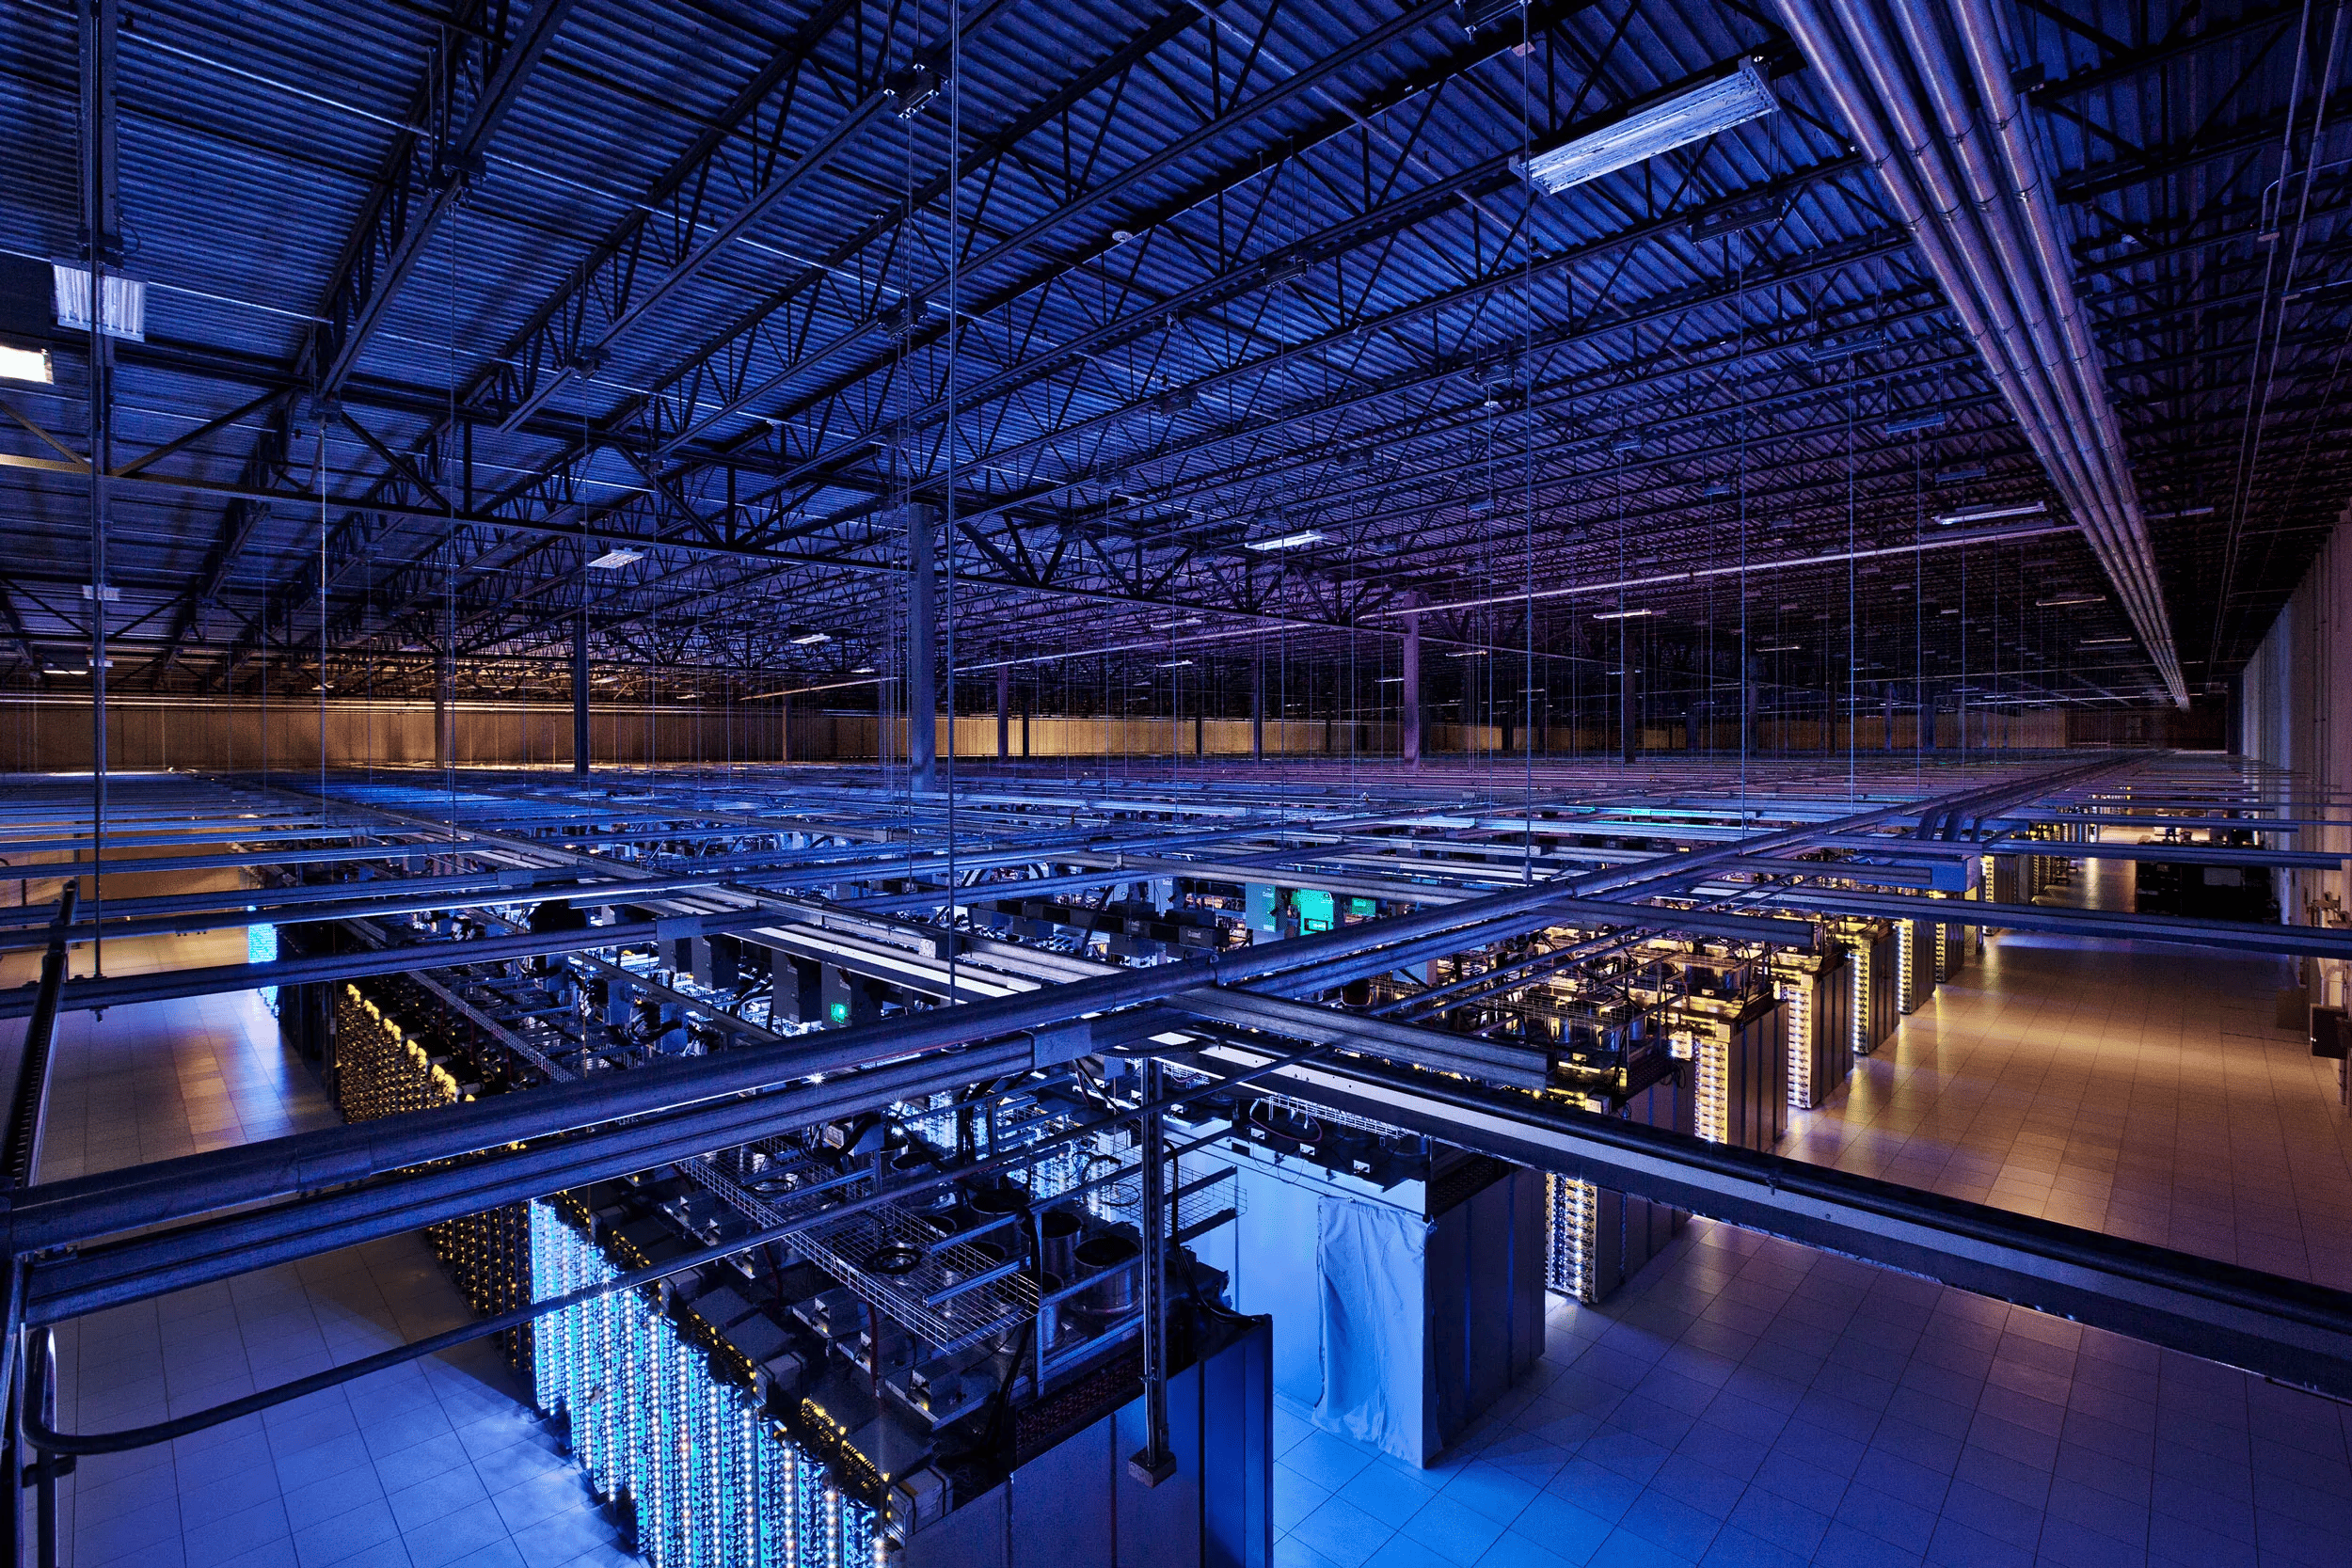
\includegraphics[width=1\textwidth]{Hinhve/data_center_energy.png}
    \caption{Trung tâm dữ liệu hiện đại với hệ thống làm mát và cơ sở hạ tầng tiêu thụ năng lượng lớn}
    \label{fig:data_center_energy}
\end{figure}

Sự phụ thuộc ngày càng tăng vào năng lượng trong mọi khía cạnh của đời sống hiện đại đã biến an ninh năng lượng thành một yếu tố quyết định sự thịnh vượng và ổn định xã hội. Các cuộc khủng hoảng năng lượng gần đây đã cho thấy tác động sâu rộng của việc gián đoạn cung cấp năng lượng đối với nền kinh tế toàn cầu. Giá cả năng lượng không chỉ ảnh hưởng trực tiếp đến chi phí sản xuất mà còn tác động đến lạm phát, tăng trưởng kinh tế và chính sách tiền tệ của các quốc gia.

Các hệ thống năng lượng hiện đại đang đối mặt với những thách thức thực tiễn cần giải pháp kỹ thuật cụ thể. Về mặt tài nguyên, sự cạn kiệt dần các nguồn năng lượng hóa thạch đang trở thành vấn đề cấp bách. Theo các ước tính hiện tại \cite{bp2023statistical}, dự trữ dầu mỏ trên thế giới chỉ còn khoảng 50 năm, khí đốt tự nhiên 52 năm và than đá 139 năm với mức tiêu thụ hiện tại. Đồng thời, sự phân bố không đều về tài nguyên năng lượng trên thế giới đã tạo ra sự phụ thuộc lẫn nhau giữa các quốc gia, dẫn đến những bất ổn địa chính trị nghiêm trọng. Chi phí khai thác cũng ngày càng tăng cao do phải tiếp cận các nguồn tài nguyên ở những vị trí khó khăn hơn, trong khi sự biến động về giá cả năng lượng liên tục ảnh hưởng đến an ninh năng lượng của từng quốc gia.

Thách thức về môi trường không kém phần nghiêm trọng khi ngành năng lượng đóng góp tới 75\% tổng lượng khí thải nhà kính toàn cầu \cite{ipcc2022mitigation}, góp phần chính vào hiện tượng biến đổi khí hậu. Tổ chức Y tế Thế giới (WHO) ước tính có đến 7 triệu người chết mỗi năm do ô nhiễm không khí \cite{who2021ambient}, chủ yếu từ việc đốt nhiên liệu hóa thạch. Việc khai thác, vận chuyển và sử dụng năng lượng hóa thạch cũng gây tổn hại nghiêm trọng đến hệ sinh thái, trong khi áp lực từ các cam kết quốc tế như Thỏa thuận Paris về giảm phát thải carbon ngày càng gia tăng \cite{unfccc2015paris}.

Từ góc độ công nghệ, nhiều quốc gia vẫn đang sử dụng hạ tầng năng lượng lạc hậu với công nghệ cũ và hiệu suất thấp. Các hệ thống năng lượng thường hoạt động độc lập, thiếu sự tích hợp thông minh và khả năng tối ưu hóa tổng thể. Việc dự báo và quản lý nhu cầu năng lượng vẫn còn nhiều khó khăn, đặc biệt là trong bối cảnh thiếu các giải pháp lưu trữ năng lượng hiệu quả cho các nguồn tái tạo có tính biến động cao.

Các công nghệ mới đang tạo ra cơ hội để giải quyết những thách thức vận hành thực tiễn trong ngành năng lượng. Chuyển đổi sang năng lượng tái tạo đang diễn ra với tốc độ chưa từng có. Năng lượng tái tạo đã trở thành nguồn năng lượng có chi phí thấp nhất tại nhiều khu vực trên thế giới \cite{irena2023renewable}, tạo động lực mạnh mẽ cho việc đầu tư và phát triển. Công suất lắp đặt năng lượng mặt trời tăng trung bình 20\% mỗi năm, trong khi năng lượng gió trên biển cũng phát triển vượt bậc với chi phí giảm 60\% trong thập kỷ qua \cite{iea2023offshore}. Một số quốc gia tiên phong như Đan Mạch đã đạt được mốc 80\% điện năng từ các nguồn tái tạo, chứng minh tính khả thi của việc chuyển đổi năng lượng toàn diện.

Đồng thời, công nghệ lưu trữ năng lượng cũng có những bước tiến đáng kể. Giá pin lithium-ion đã giảm tới 90\% từ năm 2010 \cite{bloomberg2023bnef}, làm cho việc lưu trữ năng lượng quy mô lớn trở nên khả thi về mặt kinh tế. Công nghệ lưu trữ bằng hydro xanh đang được phát triển mạnh mẽ như một giải pháp lưu trữ dài hạn, trong khi các hệ thống lưu trữ năng lượng cơ học như PHES (Pumped Hydro Energy Storage) \cite{deane2014pumped} và CAES (Compressed Air Energy Storage) \cite{chen2013compressed} cũng được mở rộng quy mô. Theo báo cáo của IEA \cite{iea2023energy_storage}, các hệ thống lưu trữ cơ học này đang đóng góp đáng kể vào việc ổn định lưới điện và tích hợp năng lượng tái tạo. Sự phát triển của lưới điện thông minh đã cho phép quản lý năng lượng phân tán một cách hiệu quả, tạo điều kiện thuận lợi cho việc tích hợp các nguồn năng lượng tái tạo.

Xu hướng phi tập trung hóa trong sản xuất năng lượng đang mang lại những cơ hội mới cho sự phát triển bền vững \cite{irena2023decentralized}. Các hệ thống năng lượng phân tán như điện mặt trời mái nhà, tuabin gió nhỏ và hệ thống lưu trữ pin đang trở thành phổ biến, cho phép người tiêu dùng vừa là người sử dụng vừa là người sản xuất năng lượng. Mô hình prosumer (producer-consumer) này \cite{parag2016prosumer} không chỉ giảm áp lực lên hệ thống điện trung tâm mà còn tăng cường khả năng phục hồi của lưới điện trước các sự cố và thiên tai. Theo nghiên cứu của Zhang và cộng sự \cite{zhang2022distributed}, các hệ thống năng lượng phân tán có thể cải thiện hiệu quả tổng thể của lưới điện lên tới 15-25\% so với các hệ thống tập trung truyền thống.

Đầu tư vào nghiên cứu và phát triển công nghệ năng lượng sạch đang đạt mức kỷ lục, với hơn 1.8 nghìn tỷ USD được đầu tư toàn cầu trong năm 2023 \cite{irena2023renewable}. Các công nghệ đột phá như pin nhiên liệu hydro\footnote{Pin nhiên liệu hydro chuyển hóa năng lượng hóa học của hydro thành điện năng thông qua phản ứng điện hóa.}, năng lượng địa nhiệt nâng cao (EGS)\footnote{EGS (Enhanced Geothermal System) là công nghệ khai thác nhiệt từ các tầng đá sâu không có nước tự nhiên bằng cách bơm nước vào tạo dòng nhiệt.} và tổng hợp hạt nhân\footnote{Tổng hợp hạt nhân (nuclear fusion) là quá trình kết hợp các hạt nhân nhẹ thành hạt nhân nặng hơn, giải phóng năng lượng lớn, mô phỏng phản ứng trong lõi Mặt Trời.} đang từng bước chuyển từ phòng thí nghiệm sang ứng dụng thương mại. Đặc biệt, sự tiến bộ trong công nghệ vật liệu và nanô-công nghệ\footnote{Nanô-công nghệ ứng dụng vật liệu ở kích thước nanomet để cải thiện tính chất và hiệu suất thiết bị năng lượng.} đang mở ra những khả năng mới cho việc nâng cao hiệu suất và giảm chi phí của các thiết bị năng lượng tái tạo.

\subsection{Chuyển đổi số và cách mạng công nghiệp 4.0}
\label{sec:digital_transformation_industry_4_0}

Cuộc cách mạng công nghiệp 4.0 đang thúc đẩy chuyển đổi số toàn diện trong ngành năng lượng, đánh dấu bước chuyển từ các hệ thống truyền thống sang môi trường số hóa tích hợp. Các công nghệ nền tảng như Internet of Things (IoT), trí tuệ nhân tạo (AI), phân tích dữ liệu lớn (Big Data Analytics) và điện toán đám mây (Cloud Computing) không chỉ cải thiện hiệu quả vận hành mà còn tạo ra những mô hình kinh doanh hoàn toàn mới, thay đổi căn bản cách thức các doanh nghiệp năng lượng tương tác với khách hàng và quản lý tài sản.

\begin{figure}
    \centering
    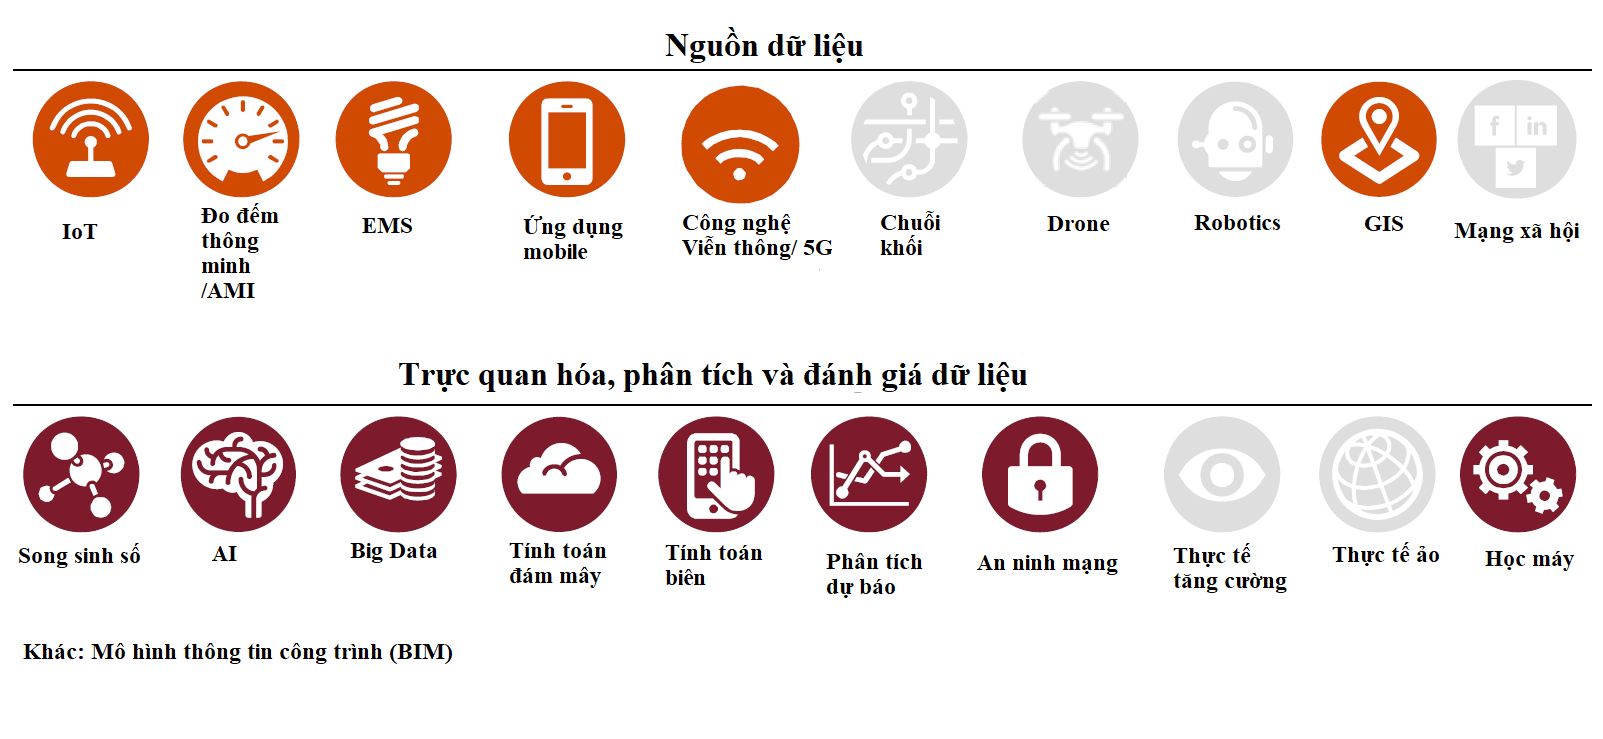
\includegraphics[width=1\textwidth]{Hinhve/digital_transformation_energy.png}
    \caption{Các công nghệ số chủ chốt (màu đậm) trong chuyển đổi số ngành năng lượng \cite{Benedettini2019EnergyDigital}}
    \label{fig:digital_transformation_energy}
\end{figure}

Chuyển đổi số trong ngành năng lượng không chỉ là một xu hướng mà đã trở thành yếu tố sống còn để duy trì khả năng cạnh tranh trong thị trường toàn cầu. Các doanh nghiệp năng lượng truyền thống đang phải tái cấu trúc mô hình hoạt động để tích hợp các công nghệ số vào mọi khâu từ thăm dò, khai thác, sản xuất đến phân phối và bán lẻ. Sự xuất hiện của các nền tảng số đã làm thay đổi cách thức giao dịch năng lượng, từ các thị trường giao ngay truyền thống sang các sàn giao dịch điện tử với khả năng thực hiện hàng triệu giao dịch mỗi giây.

Trí tuệ nhân tạo và máy học đang cách mạng hóa cách thức dự báo và quản lý trong ngành năng lượng \cite{li2023ai}. Các thuật toán AI tiên tiến có thể phân tích hàng petabyte dữ liệu để dự báo chính xác nhu cầu năng lượng với độ sai lệch dưới 1\%, tối ưu hóa việc vận hành nhà máy điện và quản lý lưới điện thông minh. Công nghệ machine learning được ứng dụng để dự đoán thời tiết, tối ưu hóa sản lượng từ các trang trại năng lượng tái tạo và thậm chí phát hiện sớm các sự cố tiềm ẩn trong hệ thống truyền tải điện.

Blockchain\footnote{Blockchain là công nghệ chuỗi khối, một dạng cơ sở dữ liệu phân tán lưu trữ thông tin trong các khối được liên kết với nhau bằng mã hóa, đảm bảo tính minh bạch và không thể thay đổi.} và các công nghệ sổ cái phân tán đang mở ra kỷ nguyên mới cho giao dịch năng lượng ngang hàng \cite{wang2023blockchain}. Các smart contract\footnote{Smart contract (hợp đồng thông minh) là chương trình máy tính tự động thực thi các điều khoản hợp đồng khi các điều kiện được đáp ứng, thường được triển khai trên nền tảng blockchain.} cho phép tự động hóa hoàn toàn việc mua bán năng lượng giữa các hộ gia đình có hệ thống điện mặt trời với nhau, loại bỏ nhu cầu trung gian và giảm chi phí giao dịch. Các đồng tiền số carbon credit đang được phát triển để tạo ra thị trường toàn cầu minh bạch và hiệu quả cho việc giao dịch quyền phát thải.

Nhu cầu thực tiễn từ doanh nghiệp tạo ra động lực mạnh mẽ cho việc ứng dụng công nghệ IoT trong quản lý năng lượng. Áp lực về hiệu quả kinh tế là động lực chính khi cạnh tranh trong thị trường năng lượng đã được tự do hóa ngày càng gay gắt. Các doanh nghiệp phải đối mặt với nhu cầu cấp thiết về giảm chi phí vận hành và bảo trì để duy trì khả năng cạnh tranh. Việc tối ưu hóa sử dụng tài sản và gia tăng tuổi thọ thiết bị trở thành yếu tố then chốt trong chiến lược kinh doanh. Đồng thời, yêu cầu minh bạch hóa thông tin cho các bên liên quan, bao gồm nhà đầu tư, cơ quan quản lý và khách hàng, cũng thúc đẩy việc ứng dụng các công nghệ số để cung cấp dữ liệu chính xác và kịp thời.

Yêu cầu về độ tin cậy và an toàn ngày càng trở nên nghiêm ngặt trong bối cảnh nhu cầu cung cấp năng lượng liên tục và ổn định. Các hệ thống năng lượng hiện đại đòi hỏi khả năng phòng ngừa và giảm thiểu rủi ro sự cố một cách chủ động thông qua các công nghệ giám sát tiên tiến. Việc tuân thủ các quy định an toàn nghiêm ngặt từ các cơ quan quản lý cũng đòi hỏi hệ thống giám sát và báo cáo tự động. Đặc biệt, trong thời đại số hóa, việc bảo vệ hạ tầng quan trọng khỏi các mối đe dọa an ninh mạng trở thành ưu tiên hàng đầu.

Sự thay đổi trong kỳ vọng của khách hàng cũng tạo ra động lực lớn cho chuyển đổi số. Khách hàng hiện đại mong muốn có nhiều lựa chọn và khả năng kiểm soát tốt hơn đối với việc sử dụng năng lượng của mình. Họ yêu cầu các dịch vụ được cá nhân hóa và khả năng tương tác số thuận tiện. Tính minh bạch trong giá cả và sự linh hoạt trong thanh toán cũng trở thành tiêu chí quan trọng. Đặc biệt, sự quan tâm ngày càng tăng đến tác động môi trường của việc tiêu thụ năng lượng đã thúc đẩy nhu cầu về các giải pháp thông minh và bền vững.

Internet of Things (IoT) trong ngành năng lượng đại diện cho một hệ sinh thái kỹ thuật số phức tạp bao gồm mạng lưới các cảm biến, thiết bị đo lường và hệ thống điều khiển thông minh được kết nối và tương tác thông qua giao thức Internet. Theo dự báo của các tổ chức nghiên cứu hàng đầu, đến năm 2025 sẽ có hơn 75 tỷ thiết bị IoT được triển khai trên toàn cầu \cite{statista2023iot}, trong đó ngành năng lượng chiếm tỷ trọng đáng kể với các ứng dụng từ giám sát thiết bị đến quản lý lưới điện thông minh. Việc ứng dụng IoT trong năng lượng tạo ra những khả năng vận hành vượt trội thông qua giám sát thiết bị thời gian thực với hàng triệu cảm biến phân bố khắp hệ thống, từ tuabin gió và tấm pin mặt trời đến máy biến áp và đường dây truyền tải. Quản lý lưới điện thông minh được hiện thực hóa thông qua các đồng hồ thông minh (smart meters) có khả năng đo lường và điều khiển dòng điện hai chiều, cho phép tích hợp hiệu quả các nguồn năng lượng phân tán. Bảo trì dự đoán trở thành khả thi và hiệu quả nhờ việc ứng dụng các thuật toán phân tích dữ liệu từ cảm biến để dự đoán chính xác thời điểm và nhu cầu bảo trì, trong khi tối ưu hóa năng lượng được thực hiện thông qua việc điều chỉnh tự động các thông số vận hành dựa trên phân tích dữ liệu thời gian thực.

Trí tuệ nhân tạo (AI) và Machine Learning đang cách mạng hóa cách thức vận hành và quản lý hệ thống năng lượng một cách toàn diện. Trong lĩnh vực dự báo nhu cầu, các thuật toán ML có thể dự báo chính xác nhu cầu điện với sai số dưới 2\%, giúp tối ưu hóa việc điều phối nguồn. AI cũng được ứng dụng để điều khiển hàng nghìn nhà máy điện nhằm tối ưu chi phí và giảm phát thải một cách đồng bộ. Công nghệ computer vision đã chứng minh hiệu quả trong việc phát hiện lỗi trên đường dây truyền tải, trong khi AI còn có khả năng thực hiện giao dịch tự động trên thị trường điện để tối ưu hóa lợi nhuận.

Big Data Analytics đóng vai trò quan trọng trong việc xử lý khối lượng dữ liệu khổng lồ mà ngành năng lượng tạo ra. Một nhà máy điện hiện đại có thể tạo ra đến 1TB dữ liệu mỗi ngày, đòi hỏi các công cụ phân tích tiên tiến. Việc phân tích hiệu suất được thực hiện thông qua xử lý dữ liệu từ hàng nghìn điểm đo để tối ưu hiệu suất vận hành. Phân khúc khách hàng dựa trên phân tích hành vi tiêu thụ giúp cung cấp dịch vụ phù hợp và cá nhân hóa. Quản lý rủi ro được cải thiện thông qua phân tích dữ liệu lịch sử để đánh giá và dự báo các rủi ro tiềm ẩn. Cuối cùng, dự báo thị trường dựa trên phân tích xu hướng giúp các doanh nghiệp đưa ra quyết định đầu tư thông minh và kịp thời.

\subsection{Tác động kinh tế và hiệu quả vận hành của IoT}
\label{sec:iot_economic_operational_impact}

\begin{figure}
    \centering
    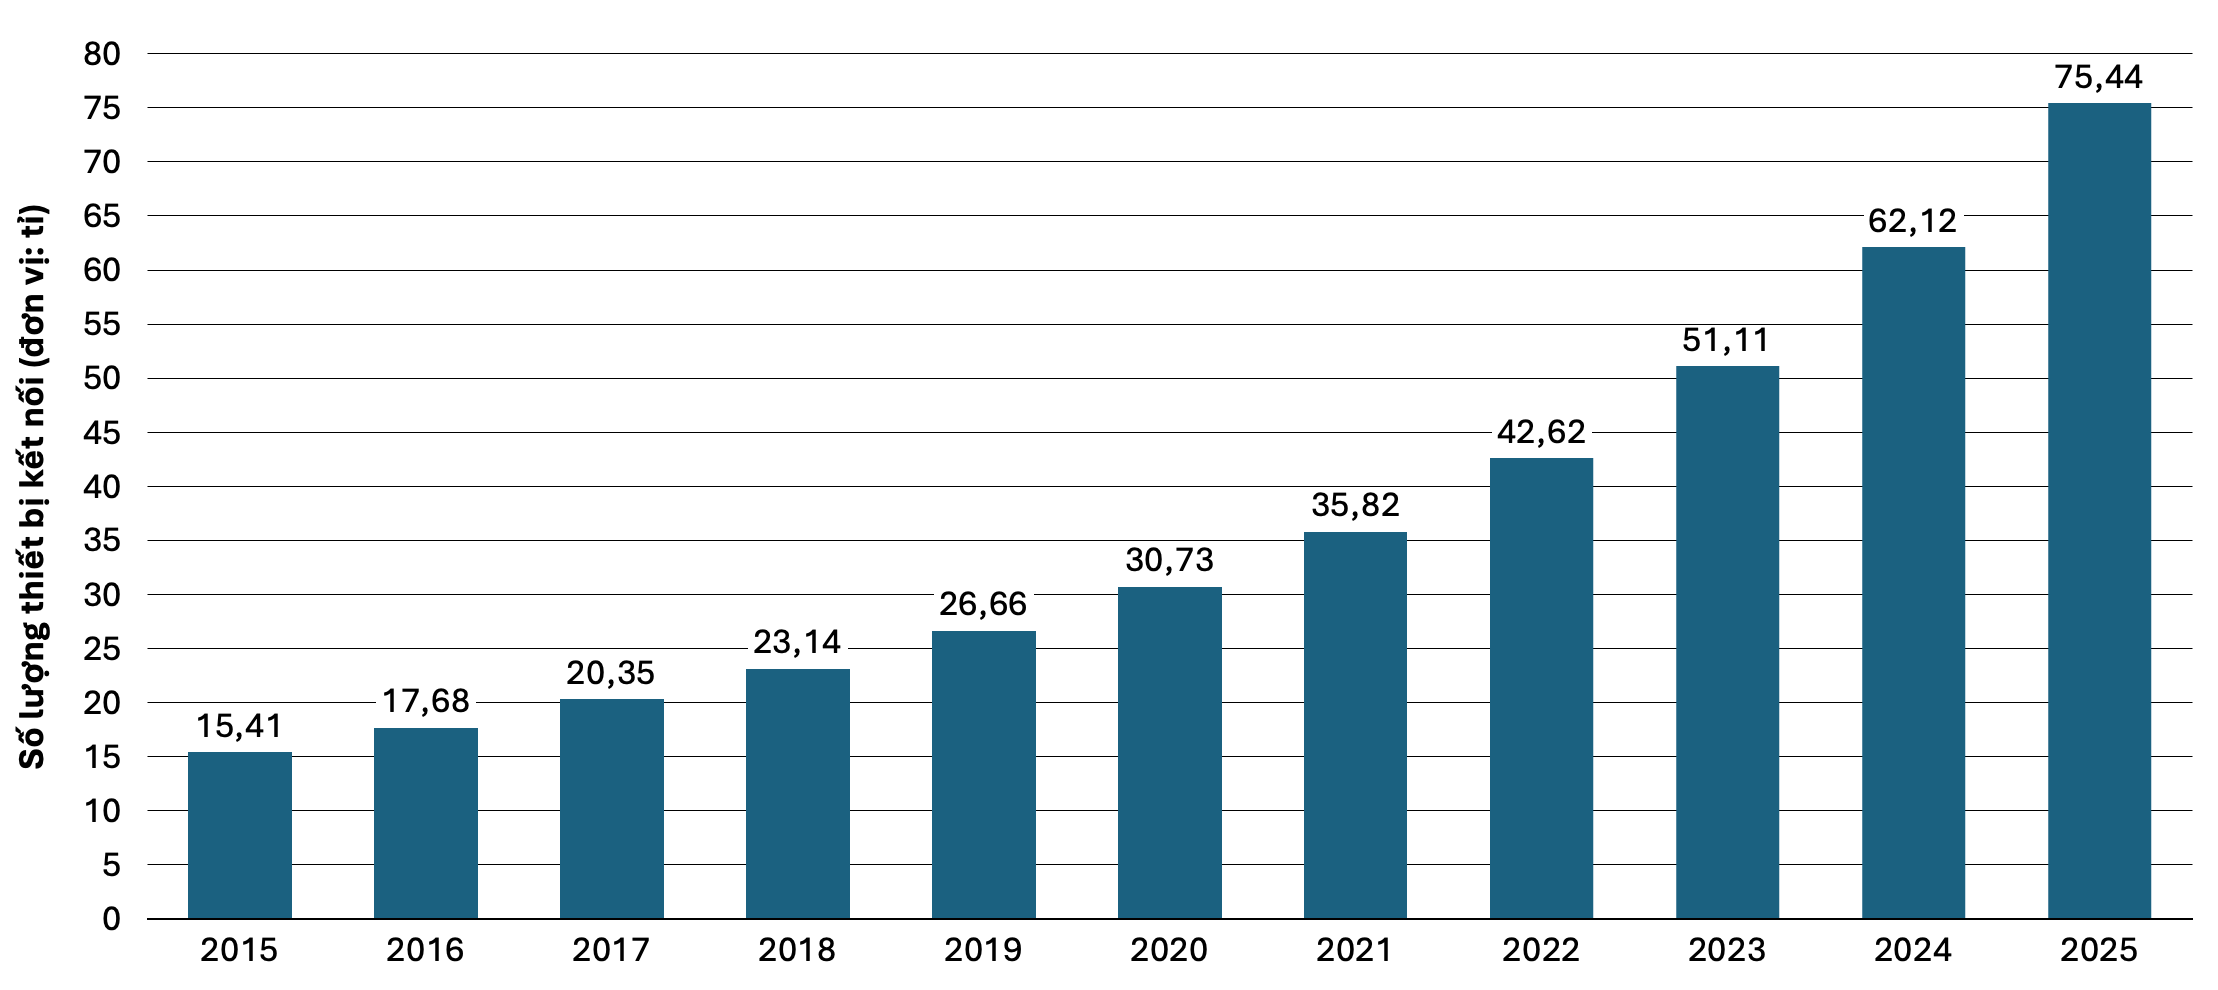
\includegraphics[width=1\textwidth]{Hinhve/iot_device.png}
    \caption{Số lượng thiết bị IoT lắp đặt trên toàn cầu từ 2015-2025 (đơn vị: tỉ) \cite{statista2023iot}}
    \label{fig:iot_device}
\end{figure}


Ứng dụng IoT trong giám sát hệ thống năng lượng mang lại lợi ích kinh tế đo lường được cho doanh nghiệp. Về mặt tiết kiệm chi phí, McKinsey ước tính rằng chuyển đổi số có thể tiết kiệm tới 80 tỷ USD mỗi năm cho ngành năng lượng toàn cầu thông qua việc tối ưu hóa vận hành và giảm lãng phí \cite{mckinsey2023digital}. Tự động hóa các quy trình vận hành có thể giảm 10-20\% chi phí vận hành nhờ việc loại bỏ các hoạt động thủ công và tăng cường hiệu quả. Đặc biệt, việc ứng dụng bảo trì dự đoán đã chứng minh khả năng giảm tới 25\% chi phí bảo trì bằng cách ngăn ngừa hỏng hóc và tối ưu hóa lịch bảo trì. Hơn nữa, các hệ thống tối ưu hóa thông minh có thể tăng 5-10\% hiệu suất thiết bị thông qua việc điều chỉnh tham số vận hành một cách liên tục và chính xác.

Chuyển đổi số đã và đang tạo ra các giá trị mới cho ngành năng lượng, góp phần thúc đẩy sự phát triển của các dịch vụ năng lượng hiện đại. Một trong những xu hướng nổi bật là sự xuất hiện của các mô hình dịch vụ năng lượng cho phép khách hàng sử dụng năng lượng linh hoạt mà không cần đầu tư lớn vào hạ tầng. Các mô hình kinh doanh dựa trên nền tảng số và hệ sinh thái số giúp kết nối nhiều chủ thể trong chuỗi giá trị năng lượng, từ nhà sản xuất, nhà cung cấp đến người tiêu dùng, qua đó tăng cường hợp tác và tối ưu hóa việc sử dụng tài nguyên. Việc khai thác dữ liệu vận hành và tiêu thụ năng lượng thông qua các công cụ phân tích chuyên sâu đã trở thành nguồn giá trị quan trọng, hỗ trợ ra quyết định và nâng cao hiệu quả kinh doanh. Bên cạnh đó, sự phát triển của các thị trường năng lượng ngang hàng cho phép các cá nhân và tổ chức thực hiện giao dịch năng lượng trực tiếp, góp phần nâng cao hiệu quả kinh tế và thúc đẩy sử dụng năng lượng tái tạo.

Giám sát IoT giúp nâng cao độ tin cậy và an toàn trong vận hành hệ thống năng lượng \cite{zhang2022iot, mckinsey2019iot}. Tối ưu hóa hệ thống được thực hiện một cách toàn diện thông qua các công nghệ thông minh \cite{zhang2022iot}. Lưới điện thông minh đã chứng minh khả năng giảm 20\% tổn thất truyền tải nhờ việc giám sát và điều khiển chính xác dòng điện \cite{iea2022smartgrid}. Việc ứng dụng AI trong tối ưu hóa lịch vận hành nhà máy điện đã giúp tiết kiệm 15\% nhiên liệu thông qua việc điều phối tối ưu các đơn vị phát điện \cite{li2023ai, mckinsey2019iot}. Hệ thống quản lý năng lượng tòa nhà thông minh có thể giảm tới 30\% tiêu thụ điện bằng cách tự động điều chỉnh các thiết bị theo nhu cầu thực tế \cite{statista2023smartbuilding, iea2022building}. Đặc biệt quan trọng, việc tích hợp năng lượng tái tạo vào lưới điện đã trở nên hiệu quả hơn 40\% nhờ các hệ thống dự báo và quản lý thông minh \cite{zhang2022distributed, irena2023decentralized}.

Độ tin cậy của hệ thống năng lượng cũng được nâng cao đáng kể. Thời gian ngừng cung cấp điện đã giảm 50\% nhờ các hệ thống giám sát và cảnh báo sớm \cite{zhang2022iot, mckinsey2019iot}. Khả năng phát hiện và khắc phục sự cố được cải thiện nhanh hơn 60\% thông qua việc ứng dụng các thuật toán thông minh và tự động hóa quy trình xử lý \cite{li2023ai, iea2022smartgrid}. Chất lượng điện năng được cải thiện đáng kể nhờ các hệ thống điều khiển tiên tiến có khả năng duy trì các thông số trong phạm vi cho phép \cite{ashrae2020powerquality}. Cuối cùng, khả năng phục hồi sau thiên tai và các sự cố lớn cũng được tăng cường thông qua việc xây dựng các hệ thống dự phòng thông minh và khả năng tái cấu hình tự động \cite{iea2023digitalization, zhao2023digital}.

\section{Công nghệ IoT và ứng dụng trong hệ thống giải nhiệt}
\label{sec:iot_technology_cooling_applications}

IoT đang được ứng dụng rộng rãi trong giám sát và tối ưu hóa hệ thống giải nhiệt công nghiệp, mang lại hiệu quả kinh tế cao và cải thiện độ tin cậy vận hành. Việc ứng dụng công nghệ IoT không chỉ giúp giảm chi phí vận hành mà còn nâng cao chất lượng dịch vụ và giảm tác động môi trường.

\begin{figure}
    \centering
    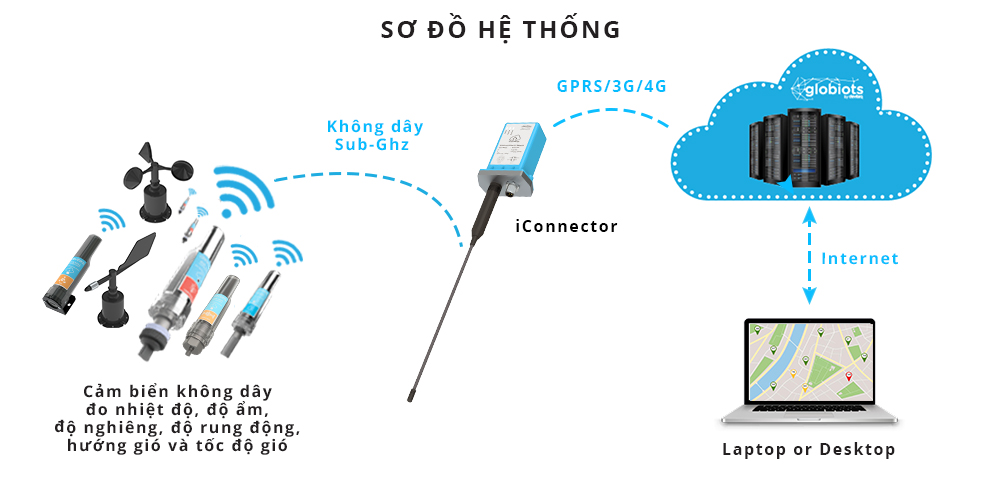
\includegraphics[width=1\textwidth]{Hinhve/iot_monitoring_system.jpg}
    \caption{Kiến trúc hệ thống giám sát IoT cho công nghiệp}
    \label{fig:iot_monitoring_system}
\end{figure}

Hệ thống giải nhiệt thông minh sử dụng IoT có khả năng giám sát liên tục các thông số vận hành như nhiệt độ, áp suất, lưu lượng và hiệu suất làm mát. Dữ liệu thời gian thực được thu thập và phân tích để tối ưu hóa hoạt động, dự đoán nhu cầu bảo trì và cảnh báo sớm các sự cố tiềm ẩn.

Sự kết hợp giữa IoT và điện toán biên (edge computing) đang tạo ra những đột phá quan trọng trong quản lý năng lượng \cite{kumar2023edge}. Thay vì phải gửi tất cả dữ liệu về trung tâm xử lý, các thiết bị IoT hiện đại có thể thực hiện xử lý và ra quyết định ngay tại chỗ, giảm độ trễ từ hàng giây xuống còn mili giây. Điều này đặc biệt quan trọng trong các ứng dụng giải nhiệt công nghiệp, nơi mà việc phản ứng nhanh có thể ngăn ngừa thiệt hại hàng triệu USD.

Công nghệ song sinh số (digital twin) đang trở thành công cụ không thể thiếu trong thiết kế và vận hành hệ thống năng lượng \cite{zhao2023digital}. Bằng cách tạo ra một bản sao ảo của hệ thống thực, các kỹ sư có thể mô phỏng và kiểm tra hàng nghìn kịch bản vận hành khác nhau mà không cần can thiệp vào hệ thống thật. Digital twin cho phép tối ưu hóa hiệu suất, dự đoán tuổi thọ thiết bị và thậm chí thiết kế lại hệ thống để đạt hiệu quả tối đa.

Xu hướng tích hợp đa nền tảng đang mở ra những khả năng mới cho việc quản lý năng lượng tổng thể \cite{mordor2023iot}. Các hệ thống IoT hiện đại không chỉ giám sát một thiết bị đơn lẻ mà có thể tích hợp dữ liệu từ hàng trăm nguồn khác nhau để tạo ra cái nhìn tổng thể về hiệu suất toàn hệ thống. Điều này cho phép phát hiện những mối tương quan phức tạp mà trước đây không thể nhận biết được.

\subsection{Phân tích nhu cầu giải nhiệt trong công nghiệp}
\label{sec:industrial_cooling_needs_analysis}

Trong các hệ thống năng lượng hiện đại, giải nhiệt là một trong những yếu tố cốt lõi đảm bảo sự ổn định, an toàn và hiệu quả hoạt động. Chi phí năng lượng dành cho làm mát thường chiếm 30-50\% tổng chi phí vận hành tại nhiều cơ sở công nghiệp.

Hệ thống giải nhiệt được ứng dụng rộng rãi trong nhiều lĩnh vực của ngành năng lượng, mỗi ứng dụng có những yêu cầu kỹ thuật riêng biệt. Nhà máy điện và trung tâm dữ liệu là hai ứng dụng chính có nhu cầu giải nhiệt lớn nhất. Trong các nhà máy nhiệt điện, hệ thống làm mát đóng vai trò then chốt trong việc duy trì hiệu suất và độ tin cậy của toàn bộ chu trình nhiệt. Bình ngưng có nhiệm vụ ngưng tụ hơi nước sau khi đi qua tuabin để tạo chân không cần thiết cho chu trình Rankine. Hệ thống giải nhiệt máy phát được thiết kế đặc biệt cho các máy phát điện công suất lớn, sử dụng hệ thống làm mát bằng khí hydro hoặc nước để duy trì nhiệt độ hoạt động tối ưu.

Trung tâm dữ liệu tiêu thụ 1-3\% tổng điện năng toàn cầu \cite{iea2022datacenter}, trong đó 30-50\% là cho làm mát. Hệ thống làm mát máy chủ trong trung tâm dữ liệu hiện đại đòi hỏi các giải pháp đa dạng từ hệ thống điều hoà không khí với các phòng lạnh cho đến giải nhiệt chất lỏng cho các cụm máy chủ mật độ cao. Mật độ nhiệt của các tủ rack tăng nhanh chóng từ mức 5kW/rack lên tới 50kW/rack, làm gia tăng áp lực lên hệ thống làm mát.

Trong ngành công nghiệp sản xuất, hệ thống giải nhiệt cũng đóng vai trò quan trọng. Ngành thép yêu cầu làm mát lò cao và lò điện để duy trì nhiệt độ vận hành tối ưu, tháp giải nhiệt cho các hệ thống tôi luyện để kiểm soát tốc độ làm nguội đạt tính chất cơ học mong muốn. Ngành hóa chất cũng cần hệ thống giải nhiệt nhằm mục đích kiểm soát động học phản ứng, cột chưng cất ngưng tụ cho quá trình tách chất. Ngành dầu khí với quy mô lớn đặt ra những thách thức đặc biệt cho hệ thống giải nhiệt từ hệ thống làm mát tinh chế đến hệ thống hoá lỏng khí tự nhiên (sản xuất LNG).

\begin{figure}[H]
    \centering
    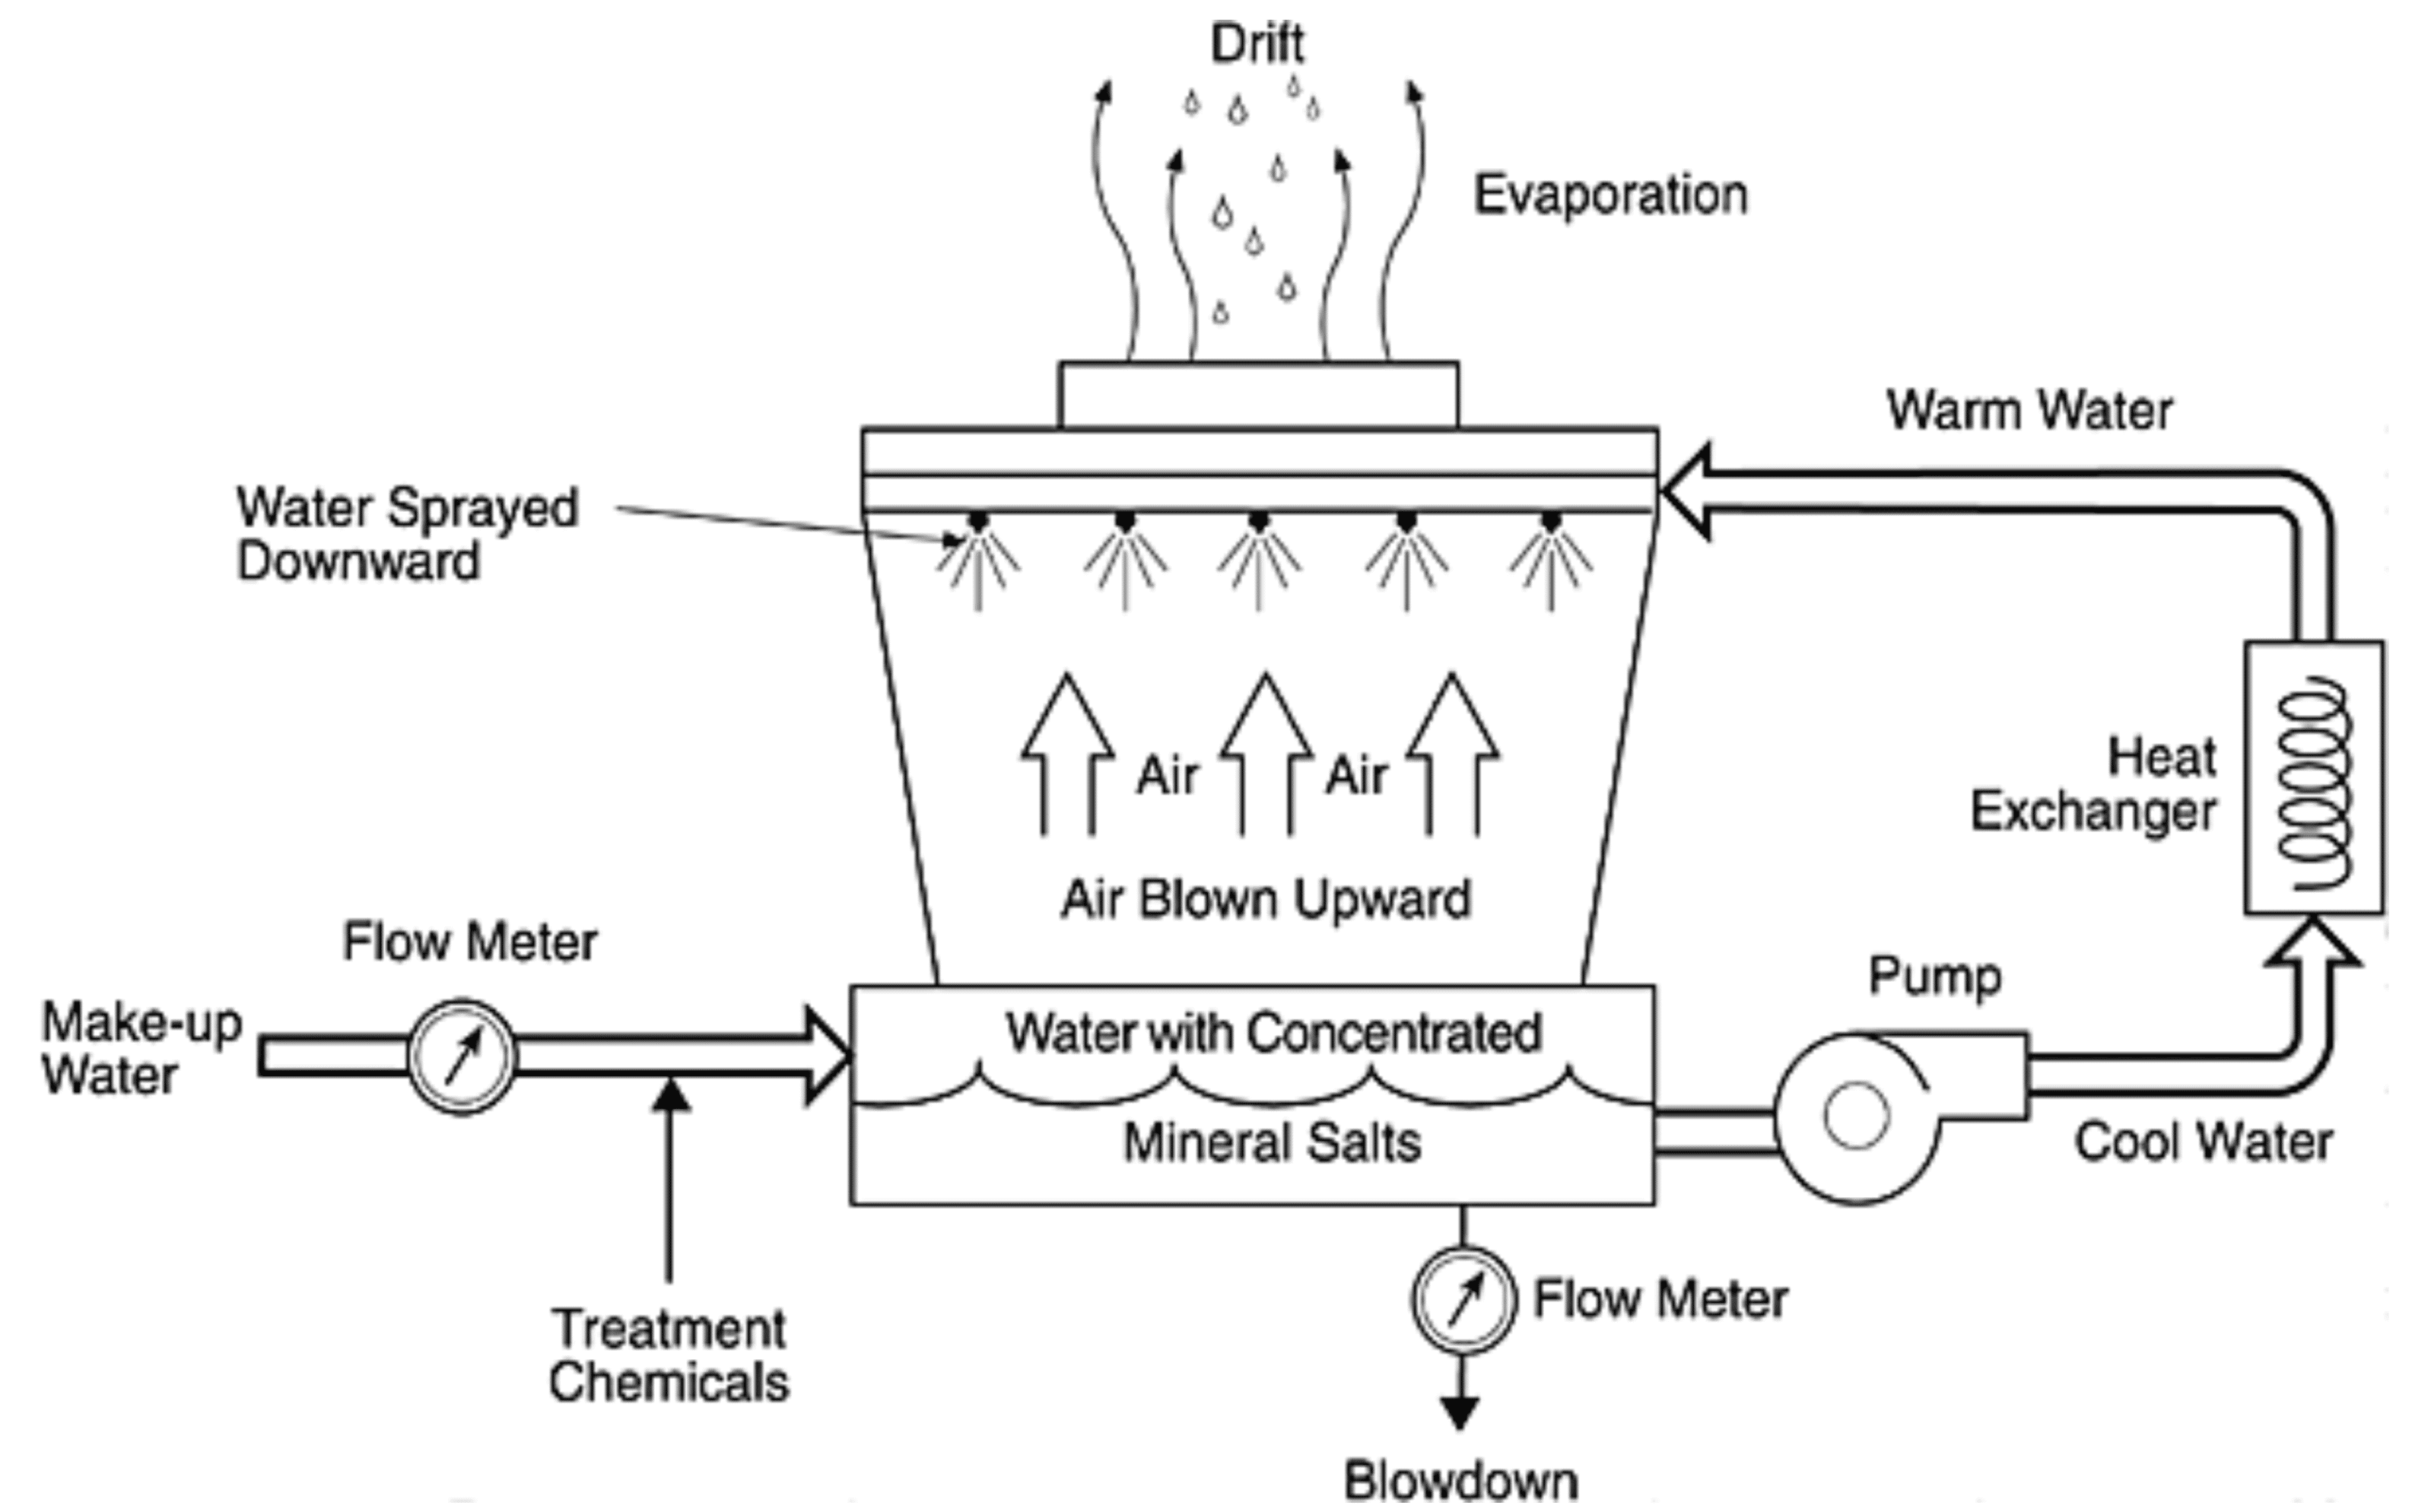
\includegraphics[width=1\textwidth]{Hinhve/gian_do_lam_mat.png}
    \caption{Giản đồ của một hệ thống nước làm mát \cite{unep2006coolingtower_en}}
    \label{fig:gian_do_lam_mat}
\end{figure}

Tháp giải nhiệt đóng vai trò trung tâm trong chu trình nhiệt công nghiệp \cite{ashrae2020cooling} với nhiều ưu điểm vượt trội. Tháp giải nhiệt có hiệu quả cao với hệ số COP (Coefficient of Performance) có thể đạt 20-40, vượt xa các phương pháp làm mát khác. Chi phí vận hành thấp do cơ cấu đơn giản và dễ bảo trì, chỉ chủ yếu tiêu thụ điện cho quạt và bơm. Khả năng xử lý nhiệt lượng rất lớn từ quy mô MW đến GW giúp đáp ứng nhu cầu của các nhà máy điện và cơ sở công nghiệp lớn. Tuổi thọ cao từ 20 đến 30 năm nếu được vận hành và bảo dưỡng đúng quy trình.

Phân loại tháp giải nhiệt được thực hiện dựa trên nhiều tiêu chí kỹ thuật khác nhau, phản ánh sự đa dạng về thiết kế và nguyên lý vận hành của thiết bị \cite{cti_cooling_towers_2011}. Một trong những tiêu chí phổ biến là phương thức tạo luồng không khí lưu thông qua tháp (phương pháp thông gió). Theo tiêu chí này, tháp giải nhiệt được chia thành loại thông gió tự nhiên và thông gió cơ học \cite{cti_cooling_towers_2011}.

Tháp giải nhiệt đối lưu tự nhiên (thường có kết cấu dạng hyperboloid) hoạt động dựa trên hiệu ứng lực đẩy nổi: sự chênh lệch nhiệt độ giữa không khí nóng bên trong tháp và không khí mát bên ngoài tạo ra dòng đối lưu đi từ đáy lên đỉnh tháp mà không cần quạt \cite{patterson_natural_draft_cooling_2013}. Loại tháp này thường có kích thước rất lớn nhằm tăng cường hiệu ứng ống khói và thường được ứng dụng trong các nhà máy điện hoặc cơ sở công nghiệp quy mô lớn. Ngược lại, tháp giải nhiệt đối lưu cơ học sử dụng các quạt công suất cao để hút hoặc đẩy không khí qua tháp, tạo ra dòng lưu thông cưỡng bức \cite{johnson_mechanical_draft_2016}. Cơ chế này giúp tăng diện tích và thời gian tiếp xúc giữa không khí với nước, nâng cao hiệu quả trao đổi nhiệt.

Bên cạnh phương thức thông gió, một tiêu chí phân loại quan trọng khác là cơ chế trao đổi nhiệt giữa nước và không khí \cite{marriott_practical_thermal_2009}. Theo đó, có hai loại chính: tháp giải nhiệt ướt (wet cooling tower) và tháp giải nhiệt khô (dry cooling tower). Tháp giải nhiệt ướt làm mát bằng quá trình bay hơi nước: nước nóng được phun thành tia hoặc màng chảy qua khối đệm, tiếp xúc trực tiếp với không khí; một phần nước bay hơi, mang theo nhiệt ẩn, phần còn lại được làm mát thông qua truyền nhiệt ẩn và truyền nhiệt hiện \cite{marriott_practical_thermal_2009}. Nhờ vậy, nhiệt độ nước có thể giảm xuống gần nhiệt độ bầu ướt của không khí môi trường. Ngược lại, tháp giải nhiệt khô truyền nhiệt chủ yếu bằng nhiệt hiện qua bề mặt trao đổi nhiệt kín, không có sự bay hơi trực tiếp, nên nhiệt độ nước sau làm mát không thể thấp hơn nhiệt độ bầu khô \cite{marriott_practical_thermal_2009}. 

Các nghiên cứu cho thấy, hệ thống giải nhiệt ướt có thể giảm tới khoảng 58\% mức tiêu thụ điện năng so với hệ thống làm mát khô tương đương \cite{ahlborn_energy_saving_2014}. Tuy nhiên, tháp ướt yêu cầu cấp nước bổ sung thường xuyên và cần xử lý nước để tránh cáu cặn, ăn mòn. Tháp khô gần như không tiêu tốn nước và ít cần bảo trì liên quan đến nguồn nước, nhưng hiệu suất làm mát thấp hơn và tiêu tốn điện năng nhiều hơn do giới hạn nhiệt độ làm mát \cite{epa_cooling_tower_guide_2017}. Vì vậy, lựa chọn giữa tháp ướt và tháp khô cần cân nhắc dựa trên yêu cầu hiệu suất, nguồn nước sẵn có, chi phí vận hành và tác động môi trường.

\begin{figure}
    \centering
    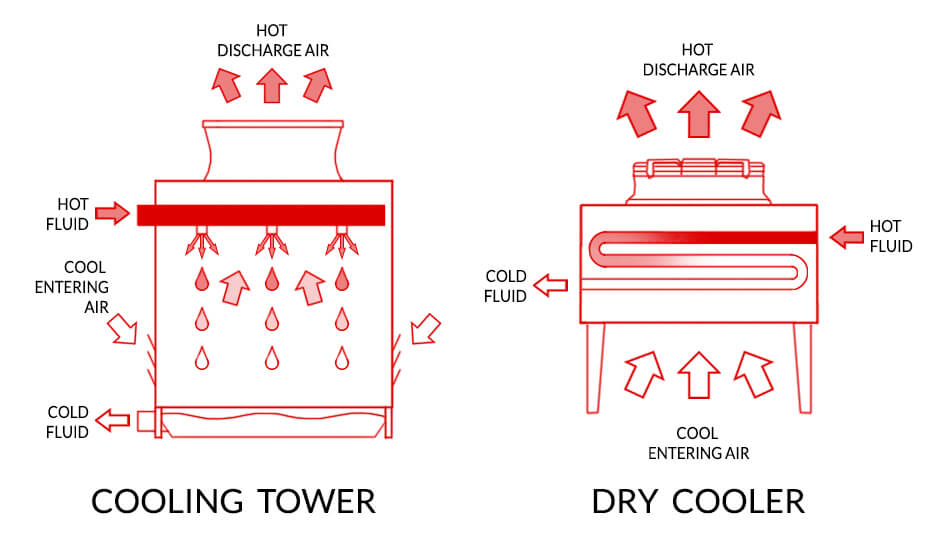
\includegraphics[width=1\textwidth]{Hinhve/dry-cooler-vs-cooling-tower.jpg}
    \caption{Tháp giải nhiệt ướt (trái) và tháp giải nhiệt khô (phải) \cite{inpart24_dry_cooler}}
    \label{fig:doi_luu_dong_ngang}
\end{figure}

Các ứng dụng giải nhiệt trong ngành năng lượng đang ngày càng đa dạng và phức tạp. Trong lĩnh vực năng lượng hạt nhân, hệ thống làm mát không chỉ đảm bảo hiệu suất vận hành mà còn đóng vai trò quan trọng trong an toàn hạt nhân. Các lò phản ứng thế hệ mới đang áp dụng công nghệ làm mát thụ động, sử dụng các nguyên lý vật lý tự nhiên để duy trì nhiệt độ an toàn ngay cả khi mất điện hoàn toàn.

Trong ngành năng lượng tái tạo, yêu cầu làm mát cũng đặt ra những thách thức riêng. Các trang trại điện mặt trời quy mô lớn cần hệ thống làm mát cho các biến tần (inverter) và hệ thống lưu trữ năng lượng. Nhiệt độ hoạt động của pin mặt trời ảnh hưởng trực tiếp đến hiệu suất, với mỗi độ C tăng lên có thể làm giảm 0.4-0.5\% công suất đầu ra. Do đó, các hệ thống làm mát tiên tiến như cooling fins thông minh và hệ thống tuần hoàn chất lỏng đang được nghiên cứu và triển khai rộng rãi.

Xu hướng thu nhỏ hoá trong công nghệ đang đặt ra những yêu cầu mới cho giải pháp làm mát. Các chip xử lý hiện đại có thể tạo ra mật độ nhiệt lên tới 1000W/cm², vượt xa khả năng của các phương pháp làm mát truyền thống. Điều này đã thúc đẩy việc phát triển các công nghệ làm mát cách mạng như làm mát chip vi kênh, làm mát bán dẫn và vật liệu biến đổi pha.

\subsection{Cách mạng hóa hệ thống quản lý năng lượng thông minh}
\label{sec:intelligent_energy_management_revolution}

Sự tích hợp sâu sắc giữa IoT và trí tuệ nhân tạo đang tạo ra cuộc cách mạng trong quản lý hệ thống giải nhiệt công nghiệp, mang lại hiệu quả vận hành vượt trội so với các phương pháp truyền thống dựa trên kinh nghiệm và điều khiển thủ công. Hệ thống giám sát thời gian thực hiện đại tạo nên nền tảng công nghệ cho quản lý giải nhiệt thông minh, trong đó mạng lưới cảm biến được triển khai dày đặc với hàng nghìn điểm đo nhiệt độ, áp suất, lưu lượng và các thông số vật lý khác được phân bố khắp toàn bộ hệ thống. Công nghệ xử lý biên (edge computing) cho phép thực hiện phân tích dữ liệu và ra quyết định điều khiển theo thời gian thực ngay tại điểm thu thập dữ liệu, giảm thiểu độ trễ và nâng cao khả năng phản ứng của hệ thống. Đặc biệt, mô hình song sinh số (digital twins) cung cấp khả năng mô phỏng và dự báo chính xác hành vi của hệ thống thực tế, hỗ trợ tối ưu hóa chủ động và triển khai chiến lược bảo trì dự đoán hiệu quả.

Lợi ích kinh tế từ việc áp dụng hệ thống làm mát thông minh thể hiện rõ nét qua khả năng tiết kiệm năng lượng đáng kể, với mức giảm tiêu thụ điện từ 20-40\% so với các hệ thống truyền thống nhờ vào việc tối ưu hóa tự động các thông số vận hành theo điều kiện thực tế. Độ tin cậy vận hành được nâng cao một cách đáng kể thông qua việc triển khai bảo trì dự đoán dựa trên phân tích dữ liệu cảm biến, giúp giảm 30-50\% thời gian ngừng hoạt động không kế hoạch và tối ưu hóa chu kỳ bảo trì. Tác động môi trường tích cực được thể hiện thông qua việc giảm dấu chân carbon từ tiết kiệm năng lượng và tối ưu hóa sử dụng tài nguyên nước trong quá trình vận hành hệ thống giải nhiệt.

Việc phát triển các công nghệ giải nhiệt thông minh, kết hợp IoT và AI, không chỉ cải thiện hiệu quả vận hành mà còn đóng góp quan trọng vào mục tiêu phát triển bền vững và trung hoà carbon của ngành năng lượng \cite{nguyen2022iot}.

Xu hướng tương lai của công nghệ giải nhiệt thông minh sẽ tập trung vào ba hướng chính: tự động hóa hoàn toàn, tích hợp đa hệ thống và bền vững môi trường. Hệ thống làm mát tự trị sử dụng AI sẽ có khả năng tự điều chỉnh, tự chẩn đoán và thậm chí tự sửa chữa mà không cần can thiệp của con người. Các thuật toán học tăng cường (reinforcement learning) sẽ cho phép hệ thống học hỏi từ kinh nghiệm và liên tục cải thiện hiệu suất theo thời gian.

Công nghệ làm mát bằng nano chất lỏng (nanofluids) đang mở ra những khả năng mới cho việc nâng cao hiệu quả truyền nhiệt \cite{chen2023nanofluids}. Bằng cách thêm các hạt nano kim loại hoặc carbon vào chất lỏng làm mát, có thể tăng hệ số dẫn nhiệt lên 20-40\% so với chất lỏng truyền thống. Điều này đặc biệt hữu ích trong các ứng dụng yêu cầu mật độ nhiệt cao như làm mát CPU và GPU thế hệ mới.

Hệ thống làm mát thích ứng (adaptive cooling) sử dụng vật liệu thông minh có khả năng thay đổi tính chất vật lý theo nhiệt độ đang được nghiên cứu tích cực \cite{pham2023adaptive}. Các vật liệu này có thể tự động điều chỉnh khả năng dẫn nhiệt hoặc thay đổi hình dạng để tối ưu hóa luồng khí, tạo ra hệ thống làm mát "sống" có thể phản ứng tự động với các thay đổi về tải nhiệt.

Xu hướng tích hợp với hệ thống quản lý năng lượng tòa nhà (Building Energy Management System - BEMS) đang trở thành tiêu chuẩn mới. Hệ thống làm mát không còn hoạt động độc lập mà được tích hợp chặt chẽ với hệ thống chiếu sáng, thông gió và các thiết bị khác để tối ưu hóa tổng thể tiêu thụ năng lượng của toàn bộ tòa nhà hoặc khu vực công nghiệp.

\subsection{Sự phát triển của các hệ thống điều khiển và giám sát công nghiệp}
\label{sec:industrial_control_monitoring_evolution}

Lịch sử phát triển của các hệ thống điều khiển và giám sát công nghiệp từ xa bắt đầu từ những năm 1990 với sự ra đời của hệ thống SCADA (Supervisory Control and Data Acquisition). Hệ thống SCADA được thiết kế như một giải pháp tập trung để điều khiển và giám sát các thiết bị công nghiệp phân tán trên diện rộng, cho phép các nhà vận hành theo dõi và điều khiển các quá trình sản xuất từ một trung tâm điều hành duy nhất \cite{boyer2009scada}.

Kiến trúc mạng của hệ thống SCADA truyền thống dựa trên mạng LAN (Local Area Network) để kết nối các thành phần với nhau, bao gồm các trạm điều khiển trung tâm, các bộ điều khiển logic khả trình (PLC), và các thiết bị đầu cuối từ xa (RTU - Remote Terminal Unit). Cấu trúc này cho phép thu thập dữ liệu từ hàng trăm điểm đo khác nhau và thực hiện điều khiển tự động dựa trên các logic được lập trình sẵn. Sự phát triển của công nghệ mạng Internet đã mở rộng khả năng của SCADA, với các nhà sản xuất PLC hàng đầu như Siemens, Allen-Bradley đã tích hợp các Web Server chuyên dụng cho phép truy cập và điều khiển hệ thống thông qua giao thức Internet Protocol.

Việc ứng dụng SCADA trong ngành công nghiệp đã mang lại những lợi ích kinh tế đáng kể và cải thiện hiệu quả vận hành toàn diện. Nâng cao năng suất sản xuất được thực hiện thông qua việc tự động hóa các quy trình và giảm thiểu thời gian chết máy do can thiệp thủ công. Chất lượng sản phẩm được cải thiện nhờ khả năng duy trì các thông số kỹ thuật ổn định và giảm biến động trong quá trình sản xuất. Chi phí vận hành và bảo trì được tối ưu hóa thông qua việc giám sát liên tục tình trạng thiết bị và thực hiện bảo trì dự đoán. Đặc biệt, việc giảm nhu cầu nhân lực trực tiếp tại hiện trường đã góp phần giảm đáng kể chi phí nhân công và nâng cao an toàn lao động trong môi trường công nghiệp nguy hiểm.

Tuy nhiên, các hệ thống SCADA truyền thống cũng bộc lộ những hạn chế nghiêm trọng trong bối cảnh công nghệ hiện đại. Tính linh hoạt trong lập trình và tùy chỉnh bị giới hạn bởi các giao diện mặc định và ngôn ngữ lập trình độc quyền của từng nhà sản xuất, tạo ra sự phụ thuộc công nghệ và hạn chế khả năng tích hợp với các hệ thống khác. Khả năng mở rộng và nâng cấp thường đòi hỏi chi phí cao và phức tạp về mặt kỹ thuật do cấu trúc khép kín của hệ thống. Giao diện người dùng thường cứng nhắc và không thể tùy chỉnh theo nhu cầu cụ thể của từng ứng dụng, làm giảm hiệu quả sử dụng và trải nghiệm người dùng.

Nhận thức về những hạn chế này đã thúc đẩy nhu cầu phát triển các giải pháp công nghệ mới có thể kế thừa những ưu điểm của SCADA trong khi khắc phục các nhược điểm cố hữu. Điều này dẫn đến sự ra đời của các nền tảng mở và linh hoạt hơn, cho phép lập trình tự do và thiết kế giao diện theo yêu cầu cụ thể mà không bị ràng buộc bởi các giới hạn của nhà sản xuất. Xu hướng này đã mở đường cho sự phát triển của công nghệ IoT hiện đại, với các vi điều khiển mã nguồn mở như ESP32, Arduino cung cấp khả năng lập trình linh hoạt và tích hợp đa dạng các giao thức truyền thông.

Sự chuyển đổi từ SCADA truyền thống sang các giải pháp IoT hiện đại không chỉ mang tính cách mạng về công nghệ mà còn thay đổi căn bản mô hình kinh doanh và vận hành trong ngành công nghiệp \cite{lee2020industry4}. Các hệ thống IoT hiện đại cung cấp khả năng tùy chỉnh cao, chi phí triển khai thấp hơn và khả năng tích hợp mượt mà với các công nghệ đám mây và phân tích dữ liệu lớn, tạo ra những cơ hội mới cho việc tối ưu hóa hiệu suất và phát triển các mô hình kinh doanh sáng tạo.

\section{Định hướng và mục tiêu ứng dụng của đề tài}
\label{sec:thesis_direction_and_application_objectives}

\subsection{Xác định bài toán thực tiễn cần giải quyết}
\label{sec:practical_problem_identification}

Trong bối cảnh chuyển đổi số và phát triển bền vững của ngành năng lượng, việc ứng dụng công nghệ IoT để giám sát và tối ưu hóa các hệ thống giải nhiệt trở nên vô cùng cấp thiết \cite{vietnam2021energy}. Các nhà máy điện, trung tâm dữ liệu và cơ sở công nghiệp hiện đang chịu áp lực ngày càng lớn về việc tiết kiệm năng lượng và giảm phát thải, không chỉ từ các quy định pháp luật mà còn từ các cam kết về phát triển bền vững của chính doanh nghiệp.

Tại Việt Nam, nhu cầu về các giải pháp giám sát và tối ưu hóa hệ thống giải nhiệt đang tăng mạnh do sự phát triển của các khu công nghiệp, trung tâm dữ liệu và nhà máy điện \cite{vietnam2021energy}. Theo báo cáo của Viện Năng lượng Việt Nam, ngành công nghiệp tiêu thụ khoảng 45\% tổng điện năng quốc gia, trong đó hệ thống làm mát chiếm tỷ trọng đáng kể. Đặc biệt, với khí hậu nhiệt đới nóng ẩm, chi phí làm mát tại Việt Nam thường cao hơn 20-30\% so với các quốc gia ôn đới.

Sự phát triển mạnh mẽ của ngành công nghệ thông tin tại Việt Nam, với việc các tập đoàn lớn như Google, Microsoft, Amazon đầu tư xây dựng trung tâm dữ liệu \cite{google2023datacenter,microsoft2023azure}, đã tạo ra nhu cầu cấp thiết về các giải pháp làm mát hiệu quả và thông minh. Các trung tâm dữ liệu này không chỉ cần đảm bảo hiệu suất cao mà còn phải tuân thủ các tiêu chuẩn quốc tế nghiêm ngặt về hiệu quả năng lượng (PUE - Power Usage Effectiveness).

\begin{figure}
    \centering
    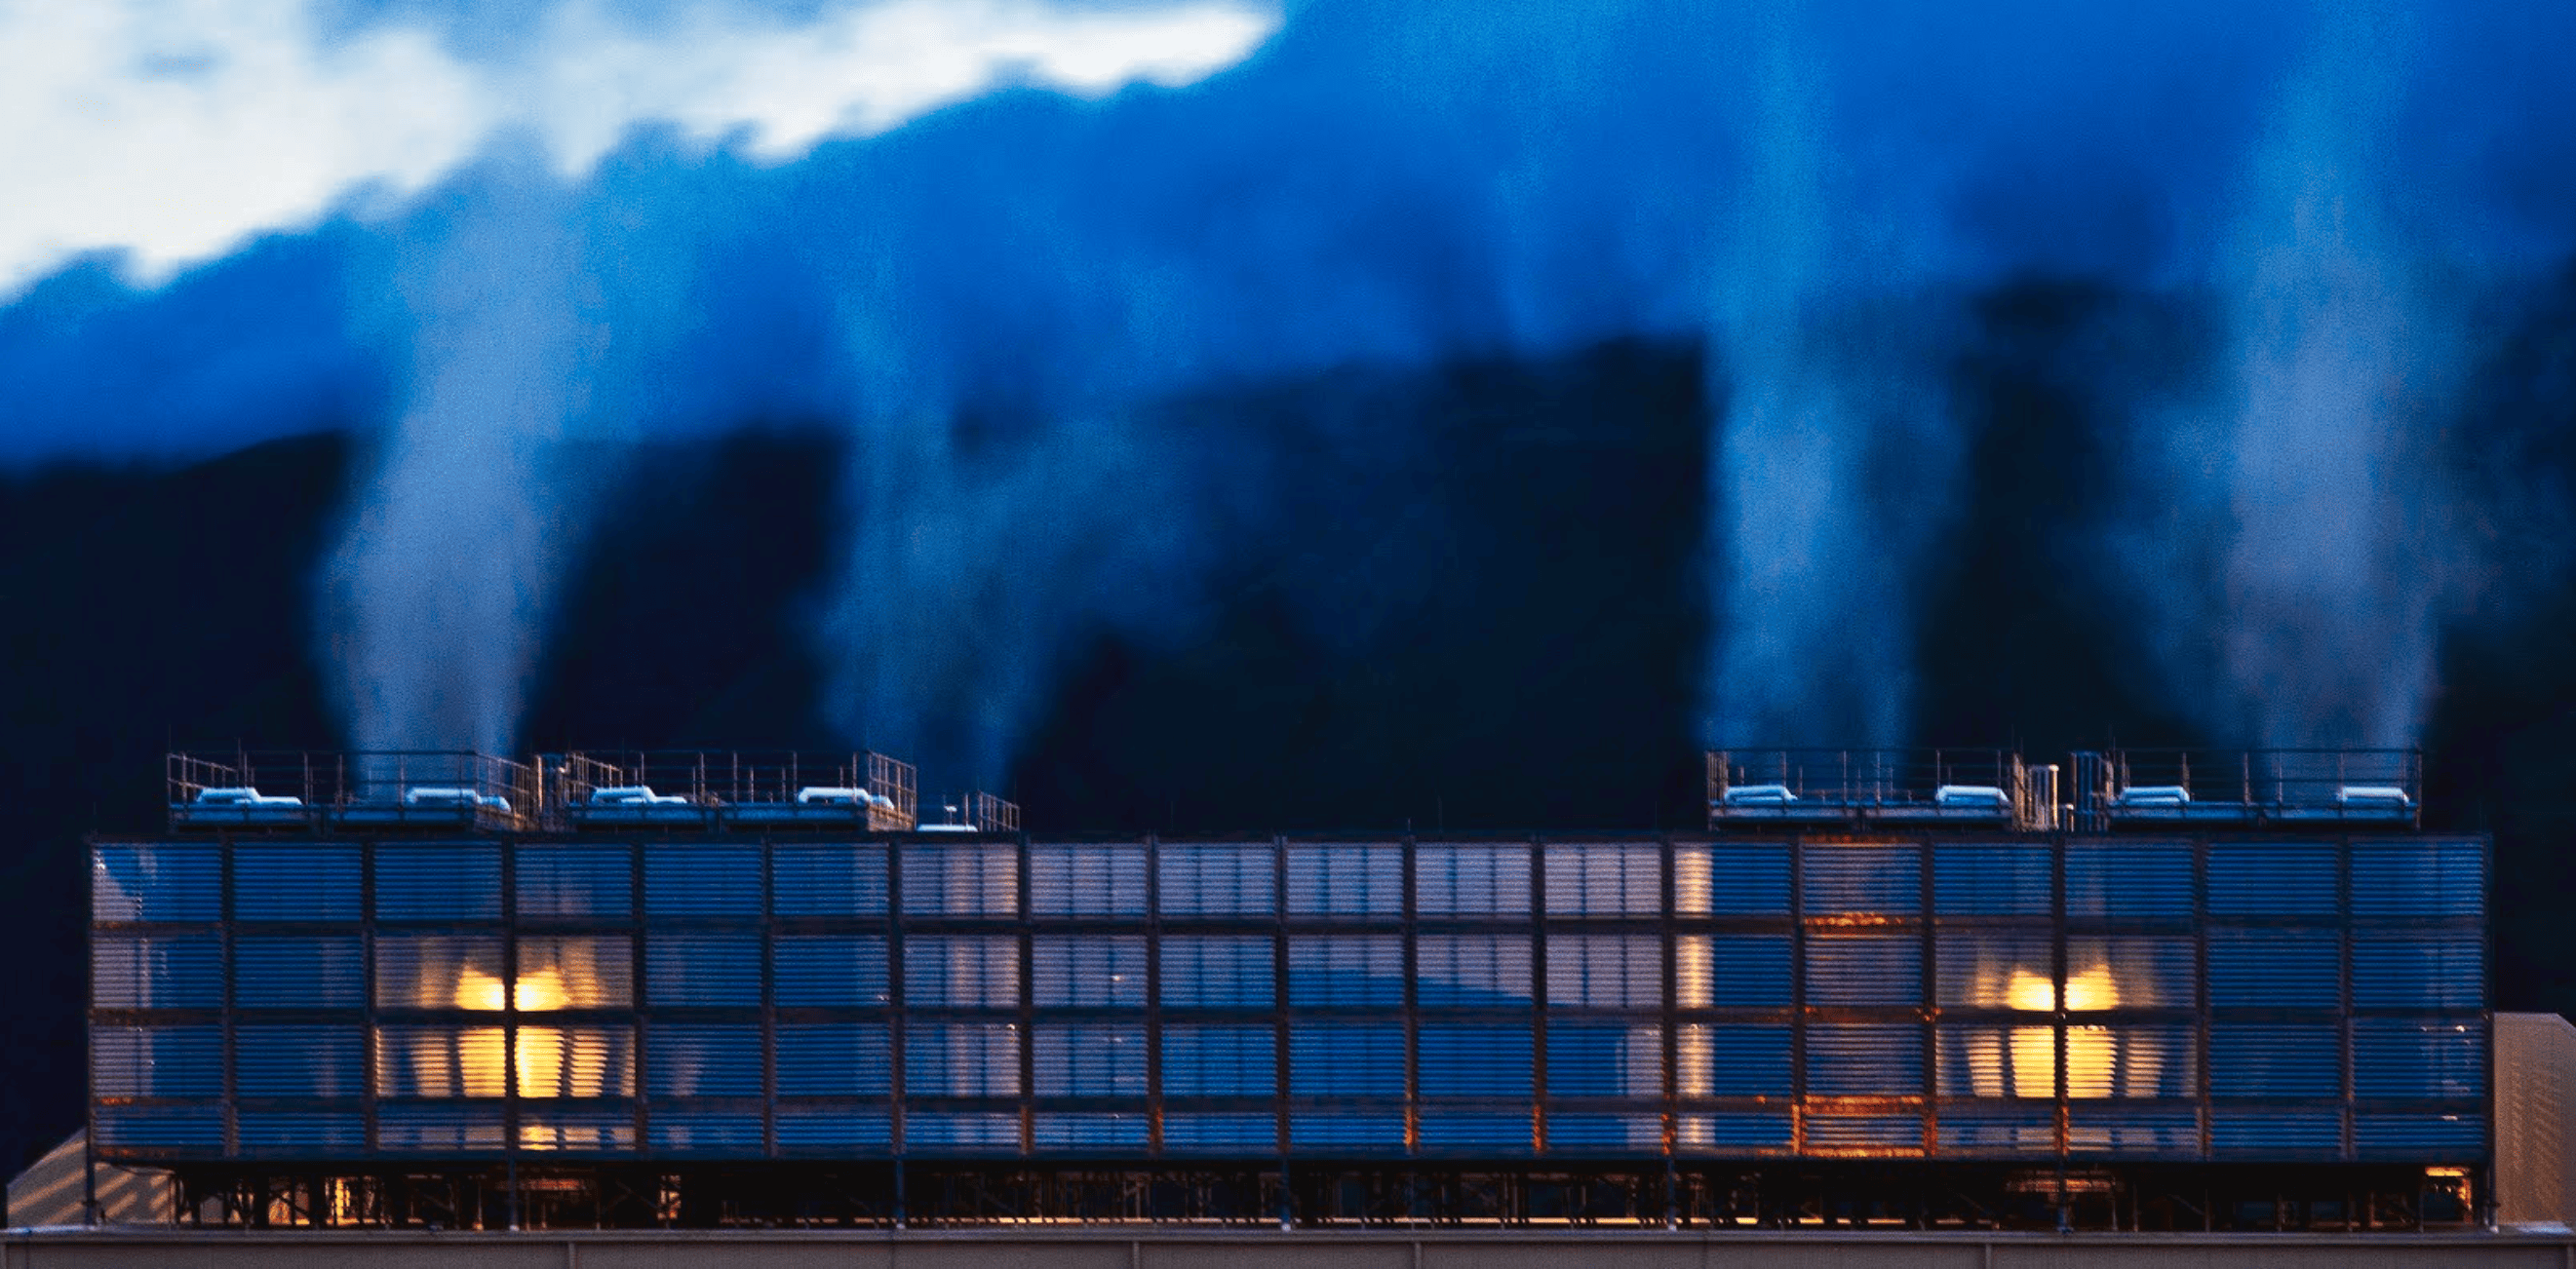
\includegraphics[width=1\textwidth]{Hinhve/google_dls_002.png}
    \caption{Hệ thống tháp giải nhiệt cho các trung tâm dữ liệu}
    \label{fig:google_dls_002}
\end{figure}

Chi phí năng lượng dành cho làm mát đã chiếm tới 30-50\% tổng chi phí vận hành hàng ngày tại nhiều cơ sở, tạo ra áp lực kinh tế đáng kể cho các doanh nghiệp. Tháp giải nhiệt, mặc dù là thiết bị quan trọng và chiếm phần lớn năng lượng tiêu thụ, nhưng thường thiếu các hệ thống giám sát thông minh và tối ưu hóa tự động. Việc vận hành không tối ưu, dựa trên kinh nghiệm và các tham số cố định, thường dẫn đến việc lãng phí năng lượng đáng kể và tăng không cần thiết chi phí bảo trì do thiếu thông tin về tình trạng thực tế của hệ thống.

\subsubsection{Các hạn chế nghiêm trọng do thiếu hệ thống giám sát}

Việc thiếu hệ thống giám sát tự động trong vận hành tháp giải nhiệt dẫn đến nhiều hậu quả nghiêm trọng về mặt kinh tế và kỹ thuật. Đầu tiên, vấn đề bảo trì thiếu khoa học là một trong những hạn chế lớn nhất. Khi không có dữ liệu thời gian thực về tình trạng thiết bị, các nhà vận hành thường áp dụng bảo trì theo lịch cố định hoặc bảo trì khắc phục sau khi sự cố đã xảy ra. Điều này dẫn đến việc thay thế linh kiện còn tốt một cách không cần thiết, hoặc ngược lại, để thiết bị hoạt động quá giới hạn an toàn gây hỏng hóc nghiêm trọng. Theo nghiên cứu của McKinsey, bảo trì dự đoán có thể giảm tới 30-50\% chi phí bảo trì so với bảo trì theo lịch trình \cite{mckinsey2023digital}.

Ảnh hưởng của yếu tố thời tiết là một thách thức lớn khác khi thiếu hệ thống giám sát tự động. Nhiệt độ và độ ẩm môi trường thay đổi liên tục trong ngày và theo mùa, trực tiếp ảnh hưởng đến hiệu suất làm mát của tháp. Trong điều kiện nhiệt độ cao và độ ẩm thấp, tháp giải nhiệt có thể hoạt động hiệu quả hơn, nhưng ngược lại trong điều kiện nóng ẩm, hiệu suất giảm đáng kể. Khi không có hệ thống điều chỉnh tự động, vận hành viên thường không kịp thời thay đổi các tham số vận hành như tốc độ quạt, lưu lượng nước tuần hoàn, dẫn đến việc tiêu thụ năng lượng không tối ưu. Nghiên cứu cho thấy sự thay đổi 5°C nhiệt độ môi trường có thể làm thay đổi hiệu suất tháp giải nhiệt lên tới 15-20\%.

Hiện tượng bám bẩn và tắc nghẽn là một vấn đề quan trọng khác thường bị bỏ qua khi thiếu giám sát liên tục. Cặn bẩn, tảo và các chất lắng đọng tích tụ dần trên bề mặt đệm làm mát, ống dẫn nước và cánh quạt. Quá trình này diễn ra từ từ và không dễ quan sát bằng mắt thường, nhưng có tác động nghiêm trọng đến hiệu suất. Lớp cặn bẩn dày chỉ 1mm có thể giảm 10-15\% khả năng truyền nhiệt. Khi không có hệ thống giám sát áp suất, nhiệt độ và lưu lượng, việc phát hiện sự suy giảm hiệu suất này thường muộn màng, khi thiệt hại đã trở nên đáng kể.

\begin{figure}
    \centering
    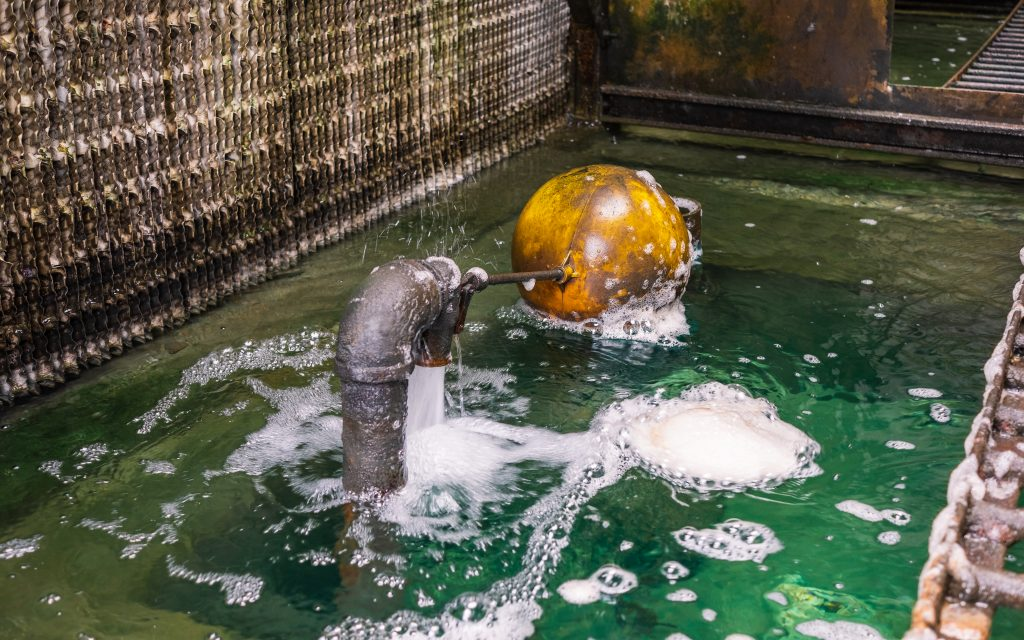
\includegraphics[width=1\textwidth]{Hinhve/dirty-cooling-tower-factory-authorized-service.jpg}
    \caption{Bám bẩn do cáu cặn trong tháp giải nhiệt}
    \label{fig:dirty-cooling-tower}
\end{figure}

Vận hành không tối ưu theo điều kiện tải là hạn chế khác của việc thiếu tự động hóa. Trong thực tế, nhu cầu làm mát thay đổi liên tục theo chu kỳ sản xuất, thời gian trong ngày và điều kiện vận hành của nhà máy. Tuy nhiên, nhiều tháp giải nhiệt được vận hành ở mức công suất cố định, thường là công suất thiết kế tối đa để đảm bảo an toàn. Điều này dẫn đến việc lãng phí năng lượng nghiêm trọng trong những thời điểm nhu cầu làm mát thấp. Ví dụ, trong ca đêm hoặc cuối tuần khi sản xuất giảm, việc duy trì tháp giải nhiệt ở công suất cao là hoàn toàn không cần thiết nhưng vẫn tiêu tốn điện năng đáng kể cho quạt và bơm nước.

Thiếu dữ liệu để phân tích và cải tiến là một hạn chế dài hạn không kém quan trọng. Khi không có hệ thống thu thập dữ liệu liên tục, các kỹ sư vận hành không thể phân tích xu hướng hiệu suất, xác định các pattern vận hành tối ưu, hay đánh giá hiệu quả của các biện pháp cải tiến. Điều này dẫn đến việc các quyết định vận hành thường dựa trên kinh nghiệm chủ quan thay vì dữ liệu khách quan, hạn chế khả năng cải thiện liên tục hiệu suất hệ thống.

Cuối cùng, rủi ro sự cố và downtime không được kiểm soát là hệ quả nghiêm trọng nhất của việc thiếu giám sát. Khi các thông số vận hành như nhiệt độ, áp suất, độ rung không được theo dõi liên tục, các dấu hiệu báo trước sự cố thường bị bỏ qua. Điều này có thể dẫn đến những sự cố nghiêm trọng như cháy motor quạt, vỡ ống dẫn nước, hoặc hư hỏng đệm làm mát, gây ngừng sản xuất và tổn thất kinh tế lớn. Trong ngành công nghiệp, mỗi giờ ngừng sản xuất có thể gây thiệt hại hàng nghìn đến hàng triệu USD tùy theo quy mô và tính chất sản xuất.

Các hệ thống giám sát tháp giải nhiệt truyền thống thường có giá thành rất đắt đỏ và đòi hỏi kiến thức chuyên sâu để cài đặt và vận hành, không phù hợp với nguồn lực của nhiều doanh nghiệp. Hiện tại vẫn thiếu các giải pháp IoT tối ưu chi phí dành riêng cho các doanh nghiệp vừa và nhỏ, những đối tượng chiếm phần lớn thị trường nhưng lại có nguồn lực đầu tư hạn chế.

\subsection{Cơ hội phát triển và tiềm năng ứng dụng IoT}
\label{sec:iot_development_opportunities}

Sự phát triển vượt bậc của công nghệ cảm biến trong thập kỷ qua đã tạo ra cơ hội độc đáo cho việc xây dựng các hệ thống giám sát thông minh với chi phí hợp lý. Cảm biến IoT hiện đại không chỉ ngày càng có giá thành rẻ hơn (giảm hơn 80\% trong 10 năm qua) mà còn có độ chính xác cao hơn và tiết kiệm năng lượng đáng kể.

Các vi điều khiển hiện đại như ESP32 đã cung cấp khả năng xử lý mạnh mẽ tương đương với các máy tính nhỏ nhưng với giá thành chỉ vài USD, cho phép thực hiện các tính toán phức tạp trực tiếp tại thiết bị. Công nghệ kết nối không dây như WiFi đã trở nên phổ biến và ổn định, cho phép triển khai các hệ thống IoT một cách linh hoạt và không cần hạ tầng cáp mạng phức tạp.

Xu hướng mã nguồn mở và bình dân hoá của công nghệ đã tạo ra cơ hội đặc biệt cho việc phát triển các giải pháp IoT dễ tiếp cận. Các platform IoT mã nguồn mở như Arduino, và các framework như InfluxDB, Grafana đang phát triển mạnh mẽ với sự đóng góp từ hàng triệu developer trên toàn thế giới. Chi phí triển khai các giải pháp IoT dựa trên mã nguồn mở đã giảm đáng kể, đôi khi chỉ bằng 5-10\% so với các giải pháp thương mại tương đương.

Sự hội tụ của các công nghệ mới như 5G, WiFi 6, và LoRaWAN đã tạo ra cơ hội đặc biệt cho việc triển khai các hệ thống IoT quy mô lớn với độ tin cậy cao. Mạng 5G với độ trễ thấp (sub-millisecond) và khả năng kết nối hàng triệu thiết bị trên km² đặc biệt phù hợp cho các ứng dụng giám sát thời gian thực trong môi trường công nghiệp khắc nghiệt.

Việt Nam đang trong giai đoạn chuyển đổi số mạnh mẽ với sự hỗ trợ của chính phủ thông qua chiến lược quốc gia về chuyển đổi số đến 2030 \cite{vietnam2023digital}. Điều này tạo ra môi trường thuận lợi cho việc phát triển và ứng dụng các giải pháp IoT trong ngành năng lượng. Các ưu đãi về thuế, hỗ trợ nghiên cứu phát triển và các chương trình đối tác công tư đang tạo điều kiện cho sự phát triển của ngành công nghệ IoT trong nước.

Xu hướng phát triển bền vững và ESG (Environmental, Social, and Governance - Môi trường, Xã hội và Quản trị) ngày càng được các doanh nghiệp chú trọng \cite{deloitte2023esg}, tạo động lực mạnh mẽ cho việc đầu tư vào các công nghệ giúp giảm tiêu thụ năng lượng và phát thải carbon. Các tập đoàn đa quốc gia hoạt động tại Việt Nam thường có các mục tiêu trung hoà carbon rất tham vọng, đòi hỏi việc áp dụng các công nghệ tiên tiến để tối ưu hóa hiệu suất năng lượng.

\subsection{Mục tiêu, phạm vi và đóng góp dự kiến của đề tài}
\label{sec:thesis_objectives_scope_contributions}

Đồ án này hướng tới việc phát triển một hệ thống giám sát thông minh cho tháp giải nhiệt ứng dụng công nghệ IoT hiện đại, với mục tiêu chính là xây dựng nền tảng công nghệ có khả năng tính toán và đánh giá hiệu suất cũng như công suất tháp giải nhiệt trong thời gian thực. Hệ thống được thiết kế để giám sát liên tục và tự động các thông số vận hành quan trọng bao gồm nhiệt độ và độ ẩm không khí môi trường, nhiệt độ nước đầu vào và đầu ra của tháp, cùng với lưu lượng nước tuần hoàn trong hệ thống nhằm tính toán chính xác hiệu suất làm mát và công suất giải nhiệt theo các phương pháp kỹ thuật tiêu chuẩn. Định hướng nghiên cứu tập trung vào việc phát triển giải pháp IoT có tính khả thi cao về mặt kinh tế, sử dụng vi điều khiển mã nguồn mở kết hợp với hệ thống cảm biến chính xác cao để tạo ra một nền tảng giám sát toàn diện nhưng vẫn đảm bảo tối ưu chi phí triển khai cho các ứng dụng thực tế trong môi trường công nghiệp.

Phạm vi nghiên cứu của đồ án bao gồm hai thành phần chính. Thứ nhất là thiết kế và triển khai hệ thống giám sát IoT thời gian thực với khả năng thu thập dữ liệu liên tục và tính toán tự động hiệu suất làm mát, công suất giải nhiệt cũng như các chỉ số hiệu quả khác theo thời gian thực. Thứ hai là chế tạo một mô hình tháp giải nhiệt mini để ứng dụng và kiểm chứng hệ thống giám sát IoT trong điều kiện thực tế, đồng thời mô phỏng và quan sát sự suy giảm công suất giải nhiệt cũng như hiệu suất làm mát theo thời gian. Mô hình này cũng cho phép nghiên cứu ảnh hưởng của các điều kiện môi trường như nhiệt độ và độ ẩm đến hiệu suất tháp giải nhiệt, từ đó tạo dữ liệu thực nghiệm để phát triển và tối ưu hóa các thuật toán tính toán.

Mô hình tháp giải nhiệt mini sẽ được thiết kế với các thành phần cơ bản của một tháp giải nhiệt thực tế bao gồm hệ thống phân phối nước, đệm làm mát, quạt thông gió và bể chứa nước, cho phép mô phỏng chân thực quá trình truyền nhiệt và truyền chất. Hệ thống sẽ tích hợp các thuật toán tính toán để đánh giá hiệu suất, bao gồm tính toán nhiệt độ bầu ướt, xác định chênh lệch nhiệt độ tiếp cận của tháp giải nhiệt, tính toán công suất giải nhiệt dựa trên lưu lượng và độ chênh nhiệt độ nước, đánh giá hiệu suất làm mát cũng như phân tích xu hướng suy giảm hiệu suất theo thời gian và điều kiện vận hành.

Đồ án dự kiến mang lại những đóng góp quan trọng về mặt kỹ thuật thông qua việc xây dựng platform giám sát IoT tổng thể sử dụng các công nghệ mã nguồn mở như ESP32, InfluxDB và Grafana, tạo ra giải pháp tối ưu chi phí có thể áp dụng rộng rãi. Việc ứng dụng và phát triển các thuật toán tính toán thời gian thực chuyên biệt cho tháp giải nhiệt, thiết kế mô hình tháp mini với khả năng mô phỏng chân thực và tích hợp hệ thống cảm biến đa thông số sẽ góp phần nâng cao hiểu biết về hiệu suất tháp giải nhiệt.

Về mặt nghiên cứu khoa học, đồ án sẽ tiến hành nghiên cứu thực nghiệm về ảnh hưởng của các điều kiện môi trường đến hiệu suất tháp giải nhiệt, phân tích và mô hình hóa sự suy giảm hiệu suất theo thời gian trong điều kiện vận hành thực tế. Đồng thời, đồ án sẽ phát triển phương pháp đánh giá hiệu suất dựa trên dữ liệu thời gian thực từ IoT và xây dựng cơ sở dữ liệu thực nghiệm về hiệu suất tháp giải nhiệt trong điều kiện khí hậu nhiệt đới, điều này có giá trị đặc biệt quan trọng cho các ứng dụng tại Việt Nam và khu vực Đông Nam Á.

Về mặt ứng dụng thực tiễn, đồ án hướng tới tạo ra giải pháp giám sát tháp giải nhiệt với chi phí đầu tư thấp, phù hợp cho các doanh nghiệp vừa và nhỏ, cung cấp công cụ đánh giá hiệu suất thời gian thực giúp tối ưu hóa vận hành và tiết kiệm năng lượng. Hệ thống cảnh báo sớm cho việc bảo trì và khắc phục sự cố tháp giải nhiệt sẽ được phát triển, tạo nền tảng cho việc nghiên cứu và phát triển các hệ thống giải nhiệt thông minh trong tương lai.

Về mặt tác động dự kiến, đồ án sẽ cung cấp một mô hình nghiên cứu hoàn chỉnh về tháp giải nhiệt, từ thiết kế phần cứng, phát triển phần mềm đến thu thập và phân tích dữ liệu thực nghiệm. Hệ thống cho phép nghiên cứu chi tiết các yếu tố ảnh hưởng đến hiệu suất làm mát và phát triển các chiến lược tối ưu hóa. Đồ án tạo ra một giải pháp có thể nhân rộng cho các cơ sở công nghiệp, trung tâm dữ liệu và nhà máy điện, với khả năng tiết kiệm 10-20\% năng lượng tiêu thụ cho làm mát và giảm đáng kể chi phí bảo trì thông qua việc phát hiện sớm các vấn đề hiệu suất. Đồ án có tính ứng dụng cao và phù hợp với xu hướng chuyển đổi số trong ngành năng lượng, góp phần nâng cao hiệu quả năng lượng và bảo vệ môi trường, đồng thời tạo ra giải pháp tối ưu chi phí cho các doanh nghiệp Việt Nam trong bối cảnh phát triển bền vững.

\end{document}